 \chapter{State of the Art}
    \label{chp:sota}
    In this Chapter, relevant State-of-the-Art algorithms, definitions and frameworks are presented. This Chapter is divided in two main sections. At first, Section \ref{sota:delay_approaches} is concerned with discussing the current existing approaches developed to tackle the problem of delays within the Reinforcement Learning framework and the most efficient algorithms that are used and have been proposed to cope with them. Afterwards, Section \ref{sota:pomdp} is dedicated to a branch of the Partially Observable MDP research and algorithms that have been instrumental for the formulation of the original proposed implementation.
    
    \section{State of the Art Approaches for Delays in RL}
        \label{sota:delay_approaches}
        In this section, three different approaches to the problem of delays are presented and their advantages and disadvantages are explained along with examples of new algorithms that have been developed using them as reference. In fact, they do not only constitute a practical mean of developing new and more efficient methods to cope with delays, but they are also instructive on a broader and conceptual way of tackling the problem of delays, which is why they are referred to as "approaches" and not as "algorithms". \newline
        In particular, Section \ref{subs:augmentedapproach} presents the Augmented-State approach, focused on including all available knowledge at each time-step in a new definition of state, denoted as extended state, which brings to the definition of a new MDP on top of the delayed one. Section \ref{subs:memorylessapproach} is instead dedicated to the Memoryless approach, based on developing Agents that learn only upon the last observed state, possibly modifying existing algorithm to align the sequence of delayed rewards; while Section \ref{subs:modelbasedapproach} is concerned with the Model-Based approach, which divides the action selection process into two steps, the first concerned on elaborating a representation of the current, unknown position of the Agent, the second provides action selection based on the aforementioned representation.
        
        \subsection{Augmented State Approach}
            \label{subs:augmentedapproach}
            The Augmented State approach is the result of a combined effort to reduce the DMDP framework (Definition \ref{def:dmdp}) to the standard undelayed MDP framework (Definition \ref{def:mdp}) with a systematic process, which, in turn, would allow for the native application of existing state-of-the-art algorithms in delayed contexts and for re-acquiring the Markov property.
            
            \subsubsection{State Augmentation for Execution Delay}
                At first, \pcite{delay:execaugment} showed that it is possible to reformulate a Constantly Delayed MDP with execution and reward delay as an undelayed MDP. This objective can be achieved by defining all the components of a new Markov Decision Process starting from the given delayed process.
                
                \begin{definition}[Augmented State Space $\mathbf{I_{a}}$]
                    \label{def:execaugmentstate}
                    Given a Constantly Delayed MDP with execution and reward delay $\langle \mathbf{S}, \mathbf{A}, p, \mathbf{R}, 0, d_a, d_r \rangle$,
                    a new augmented state space $\mathbf{I_{a}}$ can be defined as follows:
                    \[ \mathbf{I_{a}} \doteq \mathbf{S} \times \mathbf{A}^{d_a} \]
                    and each state $i^a_t$ is built from the elements of $\mathbf{S}$ and $\mathbf{A}$ in the following way:
                    \[ i_t^a = \left( s_t, a_{t-d_{a}}, a_{t-d_{a}+1}, ..., a_{t-1} \right)\]
                \end{definition}
                \noindent
                In practice, the state space $\mathbf{I_{a}}$ of the new undelayed MDP is formulated in such a way that each state contains all the available information that the Agent can have in order to plan the next action: the last observed state $s_t$ and the sequence of actions ${a_{t-d_{a}}, a_{t-d_{a}+1}, ..., a_{t-1}}$ that have been executed from $s_t$ to the current unobserved state $s_{t+d_{a}}$. Figure \ref{fig:augmented_i_a} shows how the augmented state $i_t^a$ is built. 
                \\
                As a consequence of this definition, the Reward and State-Transition Probability functions need to be defined accordingly, in order to complete the MDP framework in a consistent manner.
                
                \begin{definition}[Augmented Reward function $\mathbf{R_a}$]
                    \label{def:execaugmentreward}
                    Given a Constantly Delayed MDP with execution and reward delay $ \langle \mathbf{S}, \mathbf{A}, p, \mathbf{R}, 0, d_a, d_r \rangle$,
                    a new reward function $\mathbf{R_{a}}$ can be defined as follows:
                    \[ \mathbf{R_{a}}: \mathbf{I_{a}} \times \mathbf{A} \times \mathbf{I_{a}} \rightarrow \mathds{R}\]
                    and the values assigned by $\mathbf{R_{a}}$ can be computed in the following way:
                    \[ \mathbf{R_{a}}\left( i_t, a_{t}, i_{t+1} \right) = \mathbf{R} \left( s_t, a_{t-d_{a}}, s_{t+1} \right)\]
                \end{definition}
                \noindent
                This means that the collected reward at each step is not consequence of the chosen action $a_t$, but the result of the actually executed action $a_{t-d_{a}}$.
                
                \begin{definition}(Augmented State-Transition Probability function $p_a$)
                    \label{def:execaugmenttrans}
                    Given a Constantly Delayed MDP with execution and reward delay $\langle \mathbf{S}, \mathbf{A}, p, \mathbf{R}, 0, d_a, d_r \rangle$,
                    a new State-Transition Probability function $p_a$ can be defined as follows:
                    \[ p_a :  \mathbf{I_{a}} \times \mathbf{I_{a}} \times \mathbf{A} \rightarrow [0, 1]\]
                    and the probability values assigned by $p_a$ can be computed in the following way:
                    \[ p_a \left( i_{t+1}^a | i_t^a , a_t  \right) = p ( s_{t+1} | s_t, a_{t-d_{a}} ) \]
                \end{definition}
                \begin{figure}[t]
                    \centering
                    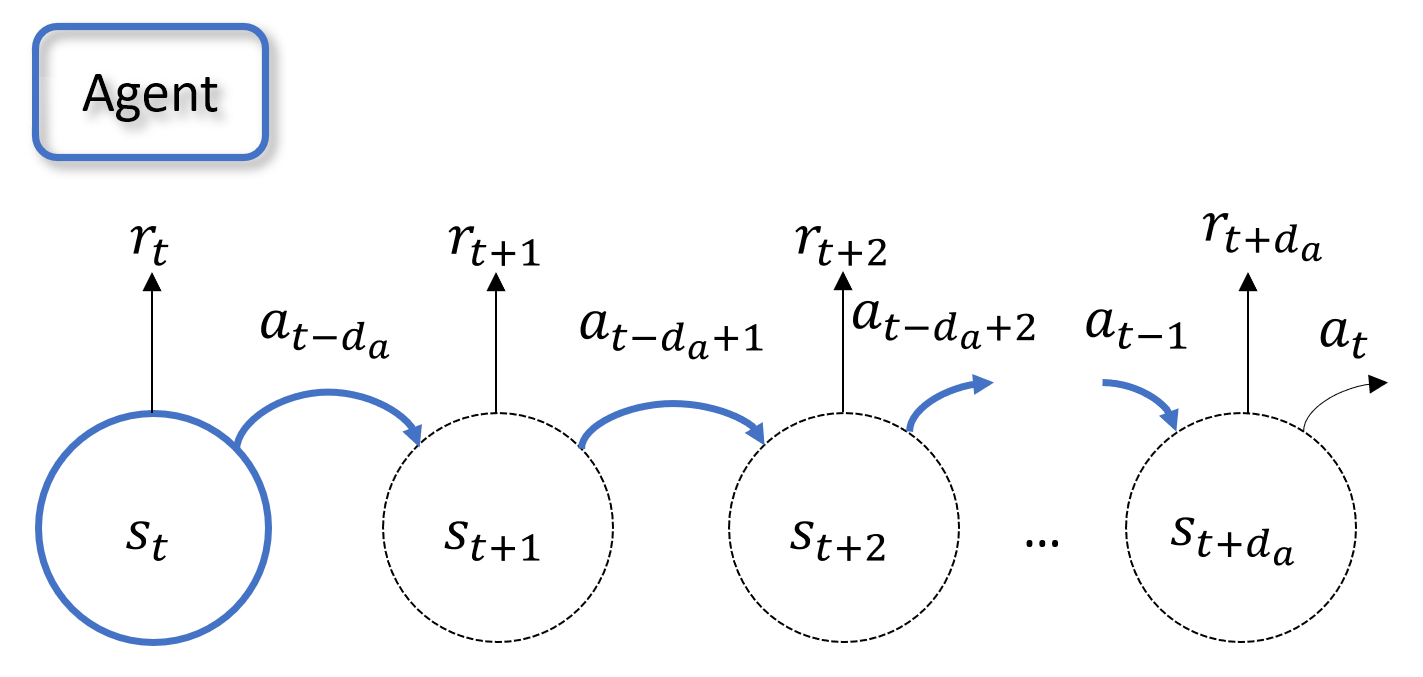
\includegraphics[width=11cm, keepaspectratio]{images/dmdp/augmented_i_a.png}
                    \caption{Augmented State $i_t^a$ is mapped onto the underlying DMDP process and it is highlighted in light blue. Reward delay is ignored for a clearer representation of the augmented state.}
                    \label{fig:augmented_i_a}
                \end{figure}
                \begin{figure}[t]
                    \centering
                    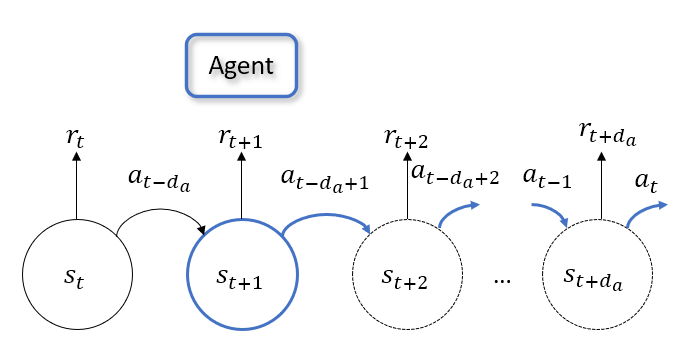
\includegraphics[width=11cm, keepaspectratio]{images/dmdp/augmented_i_a_next.png}
                    \caption{Augmented State $i_{t+1}^a$ is mapped onto the underlying DMDP and it is highlighted in light blue. Reward delay is ignored for a clearer representation of the augmented state.}
                    \label{fig:augmented_i_a_next}
                \end{figure}
                \noindent
                Again, the transition between augmented states is not the effect of the currently chosen action $a_t$, but rather of the action chosen $d_{a}$ steps before, $a_{t-d_{a}}$. This definition gives insight on how the newly formulated MDP works w.r.t. the previous DMDP framework. At a given timestep $t$, the Agent finds itself in an extended state $i_t^{a} = \left( s_t, a_{t-d_{a}}, ..., a_{t-1} \right)$ and it chooses an action $a_t$. Action $a_{t-d_{a}}$ is then executed and as consequence  the Agent finds itself a new extended state $i_{t+1}^{a} = \left( s_{t+1}, a_{t-d_{a}+1}, ..., a_{t-1}, a_{t} \right)$ with probability $p_a \left( i_{t+1}^a | i_t^a , a_t  \right)$ and collects a reward $r_t = \mathbf{R_{a}}\left( i_t, a_{t}, i_{t+1} \right)$. The new extended state $i_{t+1}^{a}$ does not contain the executed action $a_{t-d{a}}$, since the information about it is already contained in $s_{t+1}$, and it adds the selected action $a_t$ at its "tail". From a pratical point of view, the sequence of actions contained in the extended state are treated as a FIFO queue. Figure \ref{fig:augmented_i_a_next} shows the new extended state $i_{t+1}^{a}$ as a comparison against $i_t^{a}$ shown in Figure \ref{fig:augmented_i_a}.
                With all the elements presented, the main result of \pcite{delay:execaugment} can now be stated in a complete and compact way in the following theorem:
            
                \begin{theorem}[DMDP Reduction for Execution Delay]
                    \label{th:dmdpexecred}
                    A Constantly Delayed MDP with execution and reward delay $\langle \mathbf{S}, \mathbf{A}, p, \mathbf{R}, 0, d_a, d_r \rangle$ is reducible to an undelayed augmented MDP $\langle \mathbf{I_a}, \mathbf{A}, p_a, \mathbf{R_a} \rangle$ with: 
                    \begin{itemize}[topsep=0.5em, partopsep=0.5em]
                        \setlength\itemsep{0em}
                        \item $\mathbf{I_{a}} \doteq \mathbf{S} \times \mathbf{A}^{d_a}$;
                        \item $p_a \left( i_{t+1}^a | i_t^a , a_t  \right) = p \left( s_{t+1} | s_t, a_{t-d_{a}} \right)$;
                        \item $\mathbf{R_{a}}\left( i_t, a_{t}, i_{t+1} \right) = \mathbf{R} \left( s_t, a_{t-d_{a}}, s_{t+1} \right)$.
                    \end{itemize}
                \end{theorem}
                
            \subsubsection{State Augmentation for Observation Delay}
                A similar result to Theoreom \ref{th:dmdpexecred} has been achieved in a different setting. In fact, \pcite{delay:obsaugment} showed that it is possible to reduce a Constantly Delayed MDP with observation and reward delay to an undelayed MDP. This objective can be achieved by definining all the elements of the undelayed MDP starting from the ones provided by the DMDP and it is a parallel derivation to the one presented in the last section. 
                
                \begin{definition}[Augmented State Space $\mathbf{I_{o}}$]
                    \label{def:obsaugmentstate}
                    Given a Constantly Delayed MDP with observation and reward delay $\langle \mathbf{S}, \mathbf{A}, p, \mathbf{R}, d_o, 0, d_r \rangle$,
                    a new augmented state space $\mathbf{I_{o}}$ can be defined as follows:
                    \[ \mathbf{I_{o}} \doteq \mathbf{S} \times \mathbf{A}^{d_o} \]
                    and each state $i^o_t$ is built from the elements of $\mathbf{S}$ and $\mathbf{A}$ in the following way:
                    \[ i_t^o= \left( s_{t-d_{o}}, a_{t-d_{o}}, a_{t-d_{o}+1}, ..., a_{t-1} \right)\]
                \end{definition}
                \noindent
                Figure \ref{fig:augmented_i_o} shows the extended state $i_t^o$ is built starting from the DMDP elements. As in the previous section, the new extended state space is built in such a way that each state contains all the information that can be available to the Agent.
                
                \begin{definition}[Augmented Reward function $\mathbf{R_o}$]
                    \label{def:obsaugmentreward}
                    Given a Constantly Delayed MDP with observation and reward delay $ \langle \mathbf{S}, \mathbf{A}, p, \mathbf{R}, d_o, 0, d_r \rangle$,
                    a new reward function $\mathbf{R_{o}}$ can be defined as follows:
                    \[ \mathbf{R_{o}}: \mathbf{I_{o}} \times \mathbf{A} \times \mathbf{I_{o}} \rightarrow \mathds{R}\]
                    and the values assigned by $\mathbf{R_{o}}$ can be computed in the following way:
                    \[ \mathbf{R_{o}}\left( i_t, a_{t}, i_{t+1} \right) = \mathbf{E} \left[ \mathbf{R} \left( s_t, a_t, s_{t+1} | i_t \right) \right] \]
                \end{definition}
                \noindent
                Differently from the previous section, the new augmented Reward function $\mathbf{R_o}$ is defined as the expected reward over all the possible current unobserved states $s_t$ knowing the current extended state $i^o_t$, since the currently observed state $s_{t-d_{o}}$ is outdated and not involved in the current transition. 
                
                \begin{definition}(Augmented State-Transition Probability function $p_o$)
                    \label{def:obsaugmenttrans}
                    Given a Constantly Delayed MDP with execution and reward delay $\langle \mathbf{S}, \mathbf{A}, p, \mathbf{R}, d_o, 0, d_r \rangle$,
                    a new State-Transition Probability function $p_o$ can be defined as follows:
                    \[ p_o :  \mathbf{I_{o}} \times \mathbf{I_{o}} \times \mathbf{A} \rightarrow [0, 1]\]
                    and the probability values assigned by $p_o$ can be computed in the following way:
                    \[ p_o \left( i_{t+1}^o | i_t^o , a_t  \right) = p ( s_{t-d_{o}+1} | s_{t-d_{o}}, a_{t-d_{o}} ) \]
                \end{definition}                
                \noindent
                The process of transition between one extended state $i^o_t$ and its successor $i^o_{t+1}$ is completely analogous to the process presented in the last section, in State Augmentation for Execution Delay. Figure \ref{fig:augmented_i_o_next} shows the next extended state $i^o_{t+1}$ as a comparison against $i^o_t$ (Figure \ref{fig:augmented_i_o}).
                
                \begin{figure}[!b]
                    \centering
                    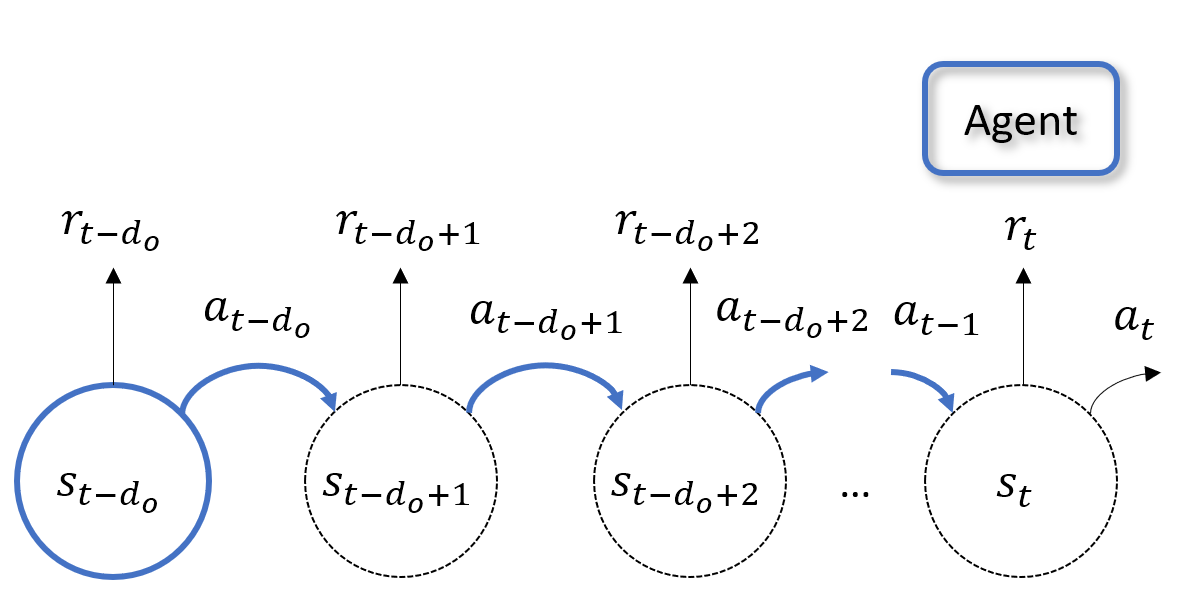
\includegraphics[width=11cm, keepaspectratio]{images/dmdp/augmented_i_o.png}
                    \caption{Augmented State $i_t^o$ is mapped onto the underlying DMDP process and it is highlighted in light blue. Reward delay is ignored for a clearer representation of the augmented state.}
                    \label{fig:augmented_i_o}
                \end{figure}
                \begin{figure}[!b]
                    \centering
                    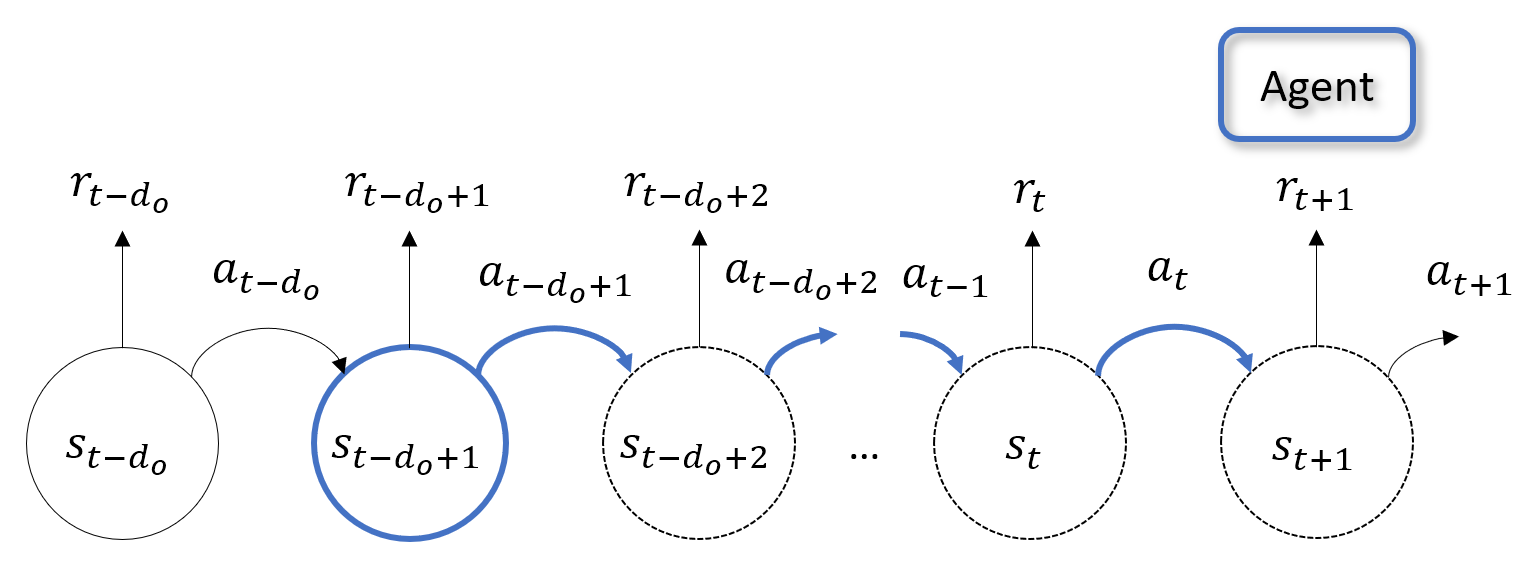
\includegraphics[width=13cm, keepaspectratio]{images/dmdp/augmented_i_o_next.png}
                    \caption{Augmented State $i_{t+1}^o$ is mapped onto the underlying DMDP and it is highlighted in light blue. Reward delay is ignored for a clearer representation of the augmented state.}
                    \label{fig:augmented_i_o_next}
                \end{figure}
                \noindent
                As in the previous section, with all the elements presented, \pcite{delay:obsaugment} result can be stated in a complete and more compact way in the following theorem:
                
                \begin{theorem}[DMDP Reduction for Observation Delay]
                    \label{th:dmdpobsred_v1}
                    A Constantly Delayed MDP with observation and reward delay $\langle \mathbf{S}, \mathbf{A}, p, \mathbf{R}, d_o, 0, d_r \rangle$ with $d_r \geq d_o$ is reducible to an undelayed augmented MDP $\langle \mathbf{I_o}, \mathbf{A}, p_o, \mathbf{R_o} \rangle$ with: 
                    \begin{itemize}[topsep=0.5em, partopsep=0.5em]
                        \setlength\itemsep{0em}
                        \item $\mathbf{I_{o}} \doteq \mathbf{S} \times \mathbf{A}^{d_o}$;
                        \item $p_o \left( i_{t+1}^o | i_t^o , a_t  \right) = p ( s_{t-d_{o}+1} | s_{t-d_{o}}, a_{t-d_{o}})$;
                        \item $\mathbf{R_{o}}\left( i_t, a_{t}, i_{t+1} \right) = \mathbf{E} \left[ \mathbf{R} \left( s_t, a_t, s_{t+1} | i_t \right) \right]$.
                    \end{itemize}
                \end{theorem}
                \noindent
                In this theorem, it is also expressed as an assumption that $d_r \geq d_o$. This is necessary due to the fact that the reward signal constitutes partial information about the transition that generated it and thus about the states that the transition involves. As stated in \pcite{delay:dmdp}, this assumption is sufficient to avoid that information about the reward signal also contains information about yet unobserved states, which would create a complex interaction between the two delayed processes.
                
            \subsubsection{Asynchronous Reward Collection}
                Before diving further into the Augmented Approach, an important intermediate result must be established in order to align the two augmentation processes presented in the last two sections. \pcite{delay:dmdp} refines the work of \pcite{delay:obsaugment} by introducing the concept of Asynchronous Reward Collection. It is shown and proved that a different and easier reward function can be used in the process of creating the Augmented MDP for Observation Delays:
                \[ \mathbf{R_{o}}\left( i^o_t, a_{t}, i^o_{t+1} \right) = \mathbf{R}\left(s_{t-d_{o}}, a_{t-d_{o}}, s_{t-d_{o}+1} \right)\]
                For a more intuitive understanding, in Figure \ref{fig:augmented_i_o}, the next collected reward would be $r_{t-d_{o}+1}$. Thus, the reward signal perceived by the Agent is the actual delayed reward signal of the original DMDP. This allows for collecting each reward exactly once and in the correct order, albeit delayed, and given that distance in time-steps between two collected rewards is the same as the distance in time-steps between the two transitions that produced them, they are also discounted properly. This property is due to the constant nature of the delays in the original CDMDP. In light of this step forward, Theorem \ref{th:dmdpobsred_v1} can be reformulated including this additional result:
                
                \begin{theorem}[DMDP Reduction for Observation Delay]
                    \label{th:dmdpobsred_v2}
                    A Constantly Delayed MDP with observation and reward delay $\langle \mathbf{S}, \mathbf{A}, p, \mathbf{R}, d_o, 0, d_r \rangle$ with $d_r \geq d_o$ is reducible to an undelayed augmented MDP $\langle \mathbf{I_o}, \mathbf{A}, p_o, \mathbf{R_o} \rangle$ with: 
                    \begin{itemize}[topsep=0.5em, partopsep=0.5em]
                        \setlength\itemsep{0em}
                        \item $\mathbf{I_{o}} \doteq \mathbf{S} \times \mathbf{A}^{d_o}$;
                        \item $p_o \left( i_{t+1}^o | i_t^o , a_t  \right) = p ( s_{t-d_{o}+1} | s_{t-d_{o}}, a_{t-d_{o}})$;
                        \item $\mathbf{R_{o}}\left( i_t, a_{t}, i_{t+1} \right) = \mathbf{R}\left(s_{t-d_{o}}, a_{t-d_{o}}, s_{t-d_{o}+1} \right)$.
                    \end{itemize}
                \end{theorem}
                \noindent
                Thanks to this last addition, the augmentation process of a CDMDP affected by observation delay is completely aligned to the augmentation process of a CDMDP affected by execution delay. This allows for the derivation of the next results for the Augmented Approach.
            
            \subsubsection{Observation and Execution Delay Equivalency}
                \label{subsubs:delayeq}
                % \begin{figure}[!t]
                %     \centering
                %     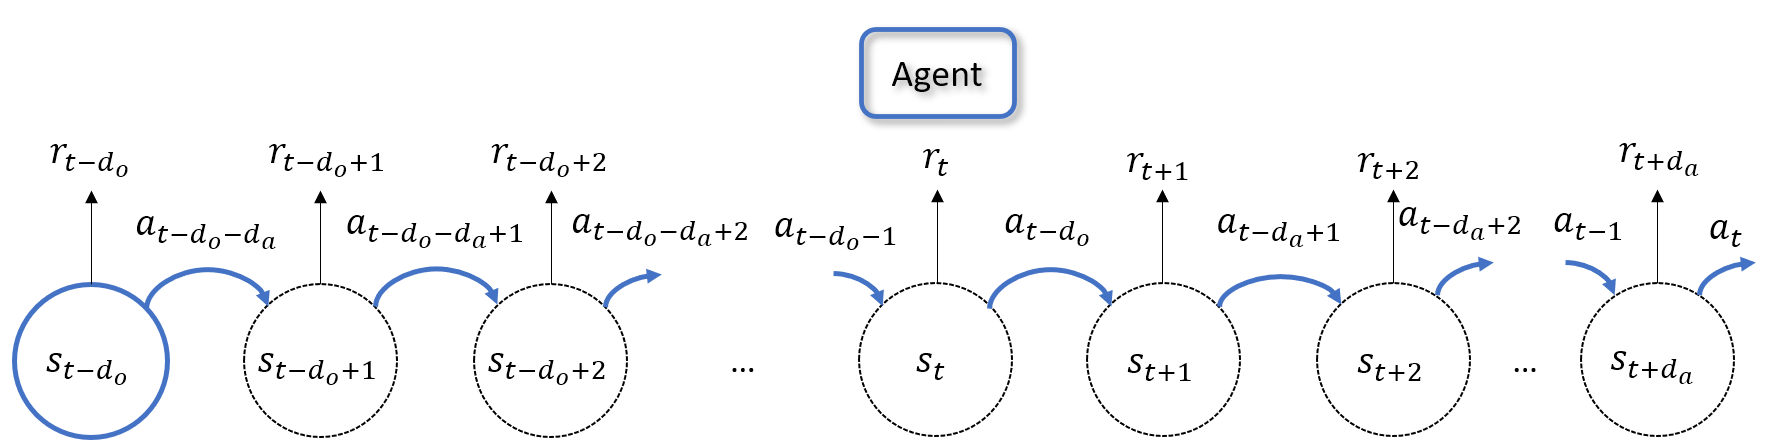
\includegraphics[width=15cm, keepaspectratio]{images/dmdp/augmented_i_ao.png}
                %     \caption{Augmented State $i_t^{ao}$ is mapped onto the underlying DMDP process and it is highlighted in light blue. Reward delay is ignored for a clearer representation of the augmented state.}
                %     \label{fig:augmented_i_ao}
                % \end{figure}
                % \begin{figure}[!t]
                %     \centering
                %     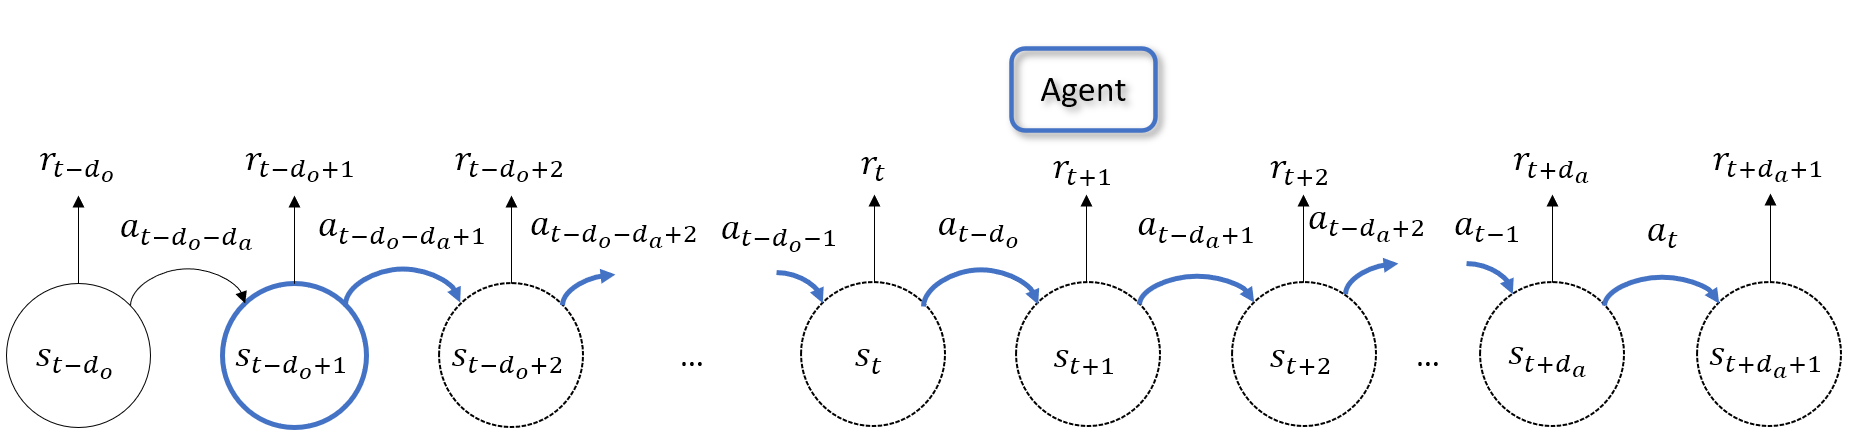
\includegraphics[width=15cm, keepaspectratio]{images/dmdp/augmented_i_ao_next.png}
                %     \caption{Augmented State $i_{t+1}^{ao}$ is mapped onto the underlying DMDP and it is highlighted in light blue. Reward delay is ignored for a clearer representation of the augmented state.}
                %     \label{fig:augmented_i_ao_next}
                % \end{figure}
                
                \pcite{delay:dmdp} stated and proved that Observation delays and Execution delays are equivalent from the perspective of the Agent and that their effect on the Augmented MDP are additive in such a way that it is possible to formulate an Augmented MDP able to express the presence of both.
                \\\\
                The equivalence of observation and execution delay can be intuitively understood by observing Figure \ref{fig:augmented_i_a} and Figure \ref{fig:augmented_i_o}. In both situations, the extended states $i^o_t$ and $i^a_t$ are constructed by using the same knowledge about the original DMDP and thus the Agent's decision-making process is based on the same notions about the Environment. The only difference between the two situations is the actual location of the Agent and thus the indexes that denotes states and actions, which is actually irrelevant to the Agent precisely because of the presence of delays. The same considerations can be made observing Figure \ref{fig:augmented_i_a_next} and Figure \ref{fig:augmented_i_o_next} and for all the pairs of future augmented states.
                \\\\
                In fact, it is easy to observe that Theorem \ref{th:dmdpexecred} and \ref{th:dmdpobsred_v2} are formally equivalent for $d_o = d_a$. Thus, even the resulting Augmented MDPs $\langle \mathbf{I_o}, \mathbf{A}, p_o, \mathbf{R_o} \rangle$ and $\langle \mathbf{I_a}, \mathbf{A}, p_a, \mathbf{R_a} \rangle$ are formally equivalent. While observation and execution delays may be consequence of different real world processes and entities, this means that they are actually perceived as the same concept, with the same consequences, for the MDP Agent that interacts in the Augumented MDP framework.
                \\\\
                Furthermore, from the equivalency of Observation and Execution delays it results that their combined effects on the Augmented MDP are additive when both are present. Supposing the presence of both observation $d_o \neq 0$ and execution delay $d_a \neq 0$, at each timestep $t$, the necessary information for optimal action selection is contained in 
                \[i_t = \left( a_{t-d_{o}-d_{a}}, a_{t-d_{o}-d_{a} +1}, ..., a_{t-d_{o}-1}, s_{t-d_{o}}, a_{t-d_{o}}, a_{t-d_{o}+1}, ..., a_{t-1} \right)\] 
                \noindent
                Afterwards, the Agent selects the action $a_t$ and finds itself in a new augmented state: 
                \[i_{t+1} = \left( a_{t-d_{o}-d_{a}+1}, a_{t-d_{o}-d_{a}+2}, ..., a_{t-d_{o}}, s_{t-d_{o}+1}, a_{t-d_{o}+1}, a_{t-d_{o}+2}, ..., a_{t-1}, a_{t}\right)\] 
                \noindent
                with probability: 
                \[p_{ao} \left( i_{t+1} | i_t, a_{t} \right) = p \left( s_{t-d_o+1} | s_{t-d_o}, a_{t-d_o-d_a} \right)\]
                \noindent
                and collecting a reward:
                \[\mathbf{R_{ao}}(i_t,a_t, i_{t+1}) = \mathbf{R}(s_{t-d_{o}}, a_{t-d_o-d_a}, s_{t-d_{o}+1})\]
                % Figure \ref{fig:augmented_i_ao} and Figure \ref{fig:augmented_i_ao_next} shows augmented states $i_t$ and $i_{t+1}$ over the underlying Constantly Delayed MDP in the case where $d_o = d_a$. 
                \noindent
                At last, in light of this result, the following complete theoreom can be stated:
                
                \begin{theorem}[CDMDP Reduction]
                    \label{th:dmdpred}
                    A Constantly Delayed MDP $\langle \mathbf{S}, \mathbf{A}, p, \mathbf{R}, d_o,$ $d_a, d_r \rangle$ with $d_r \geq d_o$ is reducible to an undelayed augmented MDP $\langle \mathbf{I_d}, \mathbf{A}, p_d, \mathbf{R_d} \rangle$ with: 
                    \begin{itemize}[topsep=0.5em, partopsep=0.5em]
                        \setlength\itemsep{0em}
                        \item $\mathbf{I_d} \doteq \mathbf{S} \times \mathbf{A}^{d_o+d_a}$;
                        \item $p_d \left( i_{t+1} | i_t, a_{t} \right) = p \left( s_{t-d_o+1} | s_{t-d_o}, a_{t-d_o-d_a} \right)$;
                        \item $\mathbf{R_d}(i_t,a_t, i_{t+1}) = \mathbf{R}(s_{t-d_{o}}, a_{t-d_o-d_a}, s_{t-d_{o}+1})$.
                    \end{itemize}
                \end{theorem}
                \noindent
                As in theorem \ref{th:dmdpobsred_v2}, the assumption $d_r \geq d_0$ is used in order to avoid situations in which the reward signal provides information about yet unobserved states. 
            
                
            \subsubsection{Approach Advantages: Markov Property and wide Applicability}
                In Section \ref{subs:markovmdp}, it is stated that the presence of delay actively hinders the Markov Property (Definition \ref{def:markov}). While the state itself still represents a sufficient statistic for the trajectory drawn before it, the fact that the Agent must plan its actions using outdated states w.r.t the actions consists in a direct violation of the Markov Property, which in turn is the foundation of the MDP framework itself, allowing for optimal action planning at each time-step. \newline
                One of the strongest advantages of the Augmented Approach is that the augmented MDP formulated from the original CDMDP retains the Markov Property. In fact, extended states are built by joining together all the information that is available for optimal action planning and the Augmented MDP does not contain any notion of delay. As a result, the Agent is interacting in a standard MDP framework, being the construction of the extended state invisible to the Agent. \newline
                Thus, any algorithm developed for interacting in the MDP framework can be used to learn the augmented MDP without any restriction. This allows state of the art algorithm to be tested directly on a delay setting without further modification to the algorithms themselves, resulting in a very large applicability of the approach. However, these benefits also comes with substantial costs.
                
            \subsubsection{Approach Disadvantages: Computational Complexity}
                While the Augmented Approach leads to a sound and complete framework that enables the possibility of acting optimally in a delayed environment, it also implies a major change in the state space in order to retain the Markov assumption. In fact, extended states are not only containing information about the environment itself, but in order to recover lost information due to delay, a sequence of actions chosen by the Agent is also added. \newline
                From the implementation point of view, the added actions function just as new dimensions for the vector or tensor that represents the extended state, which will be larger than the original state and grows larger linearly in the number of delay time-steps. Larger states usually indicate an inherently more difficult setting to learn, leading to higher variance and thus a less clear cause-effect transition. From the theoretical complexity point of view, the Augmented State Space $\mathbf{I_d}$ is much larger than the correspective State Space $\mathbf{S}$. In fact, for each state $s_t$ belonging to the original state space $\mathbf{S}$, there exist a set of extended states $i_t$ that are built from $s_t$ as a last observed state and all the possible sequences of actions of lenghts $d_o+d_a$ that are planned to be executed afterwards. This is also evident from the definition of the augmented state space: $\mathbf{I_d} \doteq \mathbf{S} \times \mathbf{A}^{d_o+d_a} \doteq \mathbf{S} \times \mathbf{A}_{1} \times \mathbf{A}_{2} \times ... \times \mathbf{A}_{d_o+d_a}$. Intuitively, the need of taking into consideration all the possible sequences of actions leads to an exponential growth in the number of delay time-steps. This intuition is taken into action in \pcite{delay:mbs}, in which a formal proof of the following theorem is provided:
                
                \begin{theorem}[Augmented State Space Complexity]
                    \label{th:dmdpobscomplexity}
                    The Augmented State Space $\mathbf{I_d}$'s cardinality of an Augmented MDP $\langle \mathbf{I_d}, \mathbf{A}, p_d, \mathbf{R_d} \rangle$ derived from a Constantly Delayed MDP $\langle \mathbf{S}, \mathbf{A}, p, \mathbf{R}, d_o, d_a, d_r \rangle$ has a lower bound of \[ | \mathbf{I_d} | = \Omega \left( | \mathbf{A}^{d_o + d_a} | \right) \]
                \end{theorem}
                \noindent
                The symbol $\Omega$ denotes the Big O notation. This result needs to be coupled with a more classical theorem that states that a MDP with fixed discount factor is solvable in polynomial time w.r.t. the State Space cardinality $| \mathbf{I_d} |$. Thus, being the State Space cardinality exponential in the length of delay $d = d_o + d_a$, the Augmented MDP can be solved in exponential time w.r.t. the length of delay $d = d_o + d_a$. This is inherently due to how the Augmented State Space $\mathbf{I_d}$ is built and it has a strong effect on applicability, since CDMDPs with relatively small delays may already be intractable in practice with the Augmented State Approach.
                
            \subsubsection{Stochastically Delayed MDP Augmentation}
                \label{subsubs:sdmdpaug}
                In the previous paragraphs of this section, the attention is posed on the CDMDP framework due to its more intuitive and less convoluted structure, that allows for presenting results in a straightforward approach. Nonetheless, equivalently important results have been derived on the Stochastically Delayed MDP framework. In fact, \pcite{delay:dmdp} also provides completely parallel results which allows for applying the Augmented State Approach also to SDMDP, with some minor but important differences.
                \\\\
                State Space Augmentation needs to take into account the fact that the Agent does not receive an observation at each time-step due to the randomness of the delay. Thus the number of dimensions of each augmented state cannot be fixed: the number of actions that occurs between one state observation and the next is variable and they all must be included in order to retain the Markov Property and optimal action selection. Each extended state is built as follows from the original SDMDP states:
                \[ i_t = \left( s_{t-d_o}, t-r, a_{t-o}, ..., a_{t-1} \right) \]
                where the execution delay $d_a$ is equal to 0 for simplicity of representation and $r$ is the number of timesteps from the last observation. Note that in this context, $d_o$ is not the constant delay but the delay sampled by the stochastic process $d_o(t)$ at time-step $t-d_o$. It is important to highlight that a variable-length extended state $i_t$ also constitutes a challenge from the algorithm's implementation perspective, since most of the algorithms that have been designed to solve MDPs have also been designed to exploit fixed-length states.
                \\\\
                An important assumption made in \pcite{delay:dmdp} is that state $s_{t+1}$ can be observed only after the observation of state $s_t$, which is coupled with the usual constraint $d_o > d_r$ to ensure that the reward result of the $t+1$ timestep can be collected only after the observation of the state $s_{t+1}$, in order not to reveal any conflicting information about the state itself. These assumptions have substantial consequences upon the Augmented State-Transition probability function, which forces the extended state to grow indefinitely large with time.
                \begin{definition}(Augmented State-Transition function $p_d$ (SDMDP))
                    \label{def:sdmdpaugtrans}
                    \[ p_d \left( i_{t+1} | i_t, a_t \right) =  
                        \begin{cases} 
                            p \left( s_{t-d_o+1} | s_{t-d_o}, a_{t-d_o} \right) q\left(r\right) & if \; i_{t+1} = i \\
                            1 - q\left(r\right) & if \; i_{t+1} = i'\\
                        \end{cases}
                    \]
                    where:
                \end{definition}
                \begin{itemize}[topsep=0.5em, partopsep=0.5em]
                    \setlength\itemsep{0em}
                    \item $q(r) = \mathds{P}\left( d_o(t) = r \right) /\; \mathds{P}\left( d_o(t) \geq r \right) $ represents the probability that the new state $s_{t-d_o+1}$ is observed in the next timestep $t+1$, given that currently observed state $s_{t-d_o}$ has been first observed $t-r$ timesteps before.
                    \item $i = \left( s_{t-d_o+1}, t+1, a_{t-d_o+1}, ..., a_{t}\right)$ is the extended state the Agent will find itself in if $s_{t-d_o+1}$ is observed at timestep $t+1$.
                    \item $i' = \left( s_{t-d_o}, t-r+1, a_{t-o}, ..., a_{t-1}, a_{t} \right)$  is the extended state the Agent will find itself in if no new state is observed at timestep $t+1$.
                \end{itemize}
                This definition of State-Transition Probability function implies that, at each timestep, the augmented state's dimensions can either remain constant or grow exactly by 1. In turn, this means that the augmented state will grow indefinitely with time if the Agent is not halted in order to wait for new observations without acting further, so to shrink the extended state to an acceptable size.
                \\\\
                The Augmented Reward Function also needs to take into account that the number of steps between observations is not constant and thus the reward signal needs to be assigned to a transition happened a variable number of steps before and avoid repeating the last reward signal at each timestep in which no new state is observed. Suppose the current extended state is $i_t = \left( s_{t-d_o}, t-r, a_{t-o}, ..., a_{t-1} \right)$ and that state $s_{t-d_o+1}$ is the next observed state, then the Reward function is defined as:
                \begin{definition}(Augmented Reward Function $\mathbf{R_d}$ (SDMDP))
                    \label{def:sdmdpaugrew}
                    \[ \mathbf{R_d} \left( i_t, a_t, i_{t+1} \right) =  
                        \begin{cases} 
                            \mathbf{R} \left( s_{t-d_o}, a_{t-d_o}, s_{t-d_o+1} \right) & if \; i_{t+1} = i \\
                            0 & if \; i_{t+1} = i'\\ 
                        \end{cases}
                    \]
                where $i$ and $i'$ are defined as in Definition \ref{def:sdmdpaugtrans}.
                \end{definition}
                \noindent
                At last, the effect of the presence of Execution Delay $d_a(t)$ is completely analogous to the CDMDP framework: 
                \begin{itemize}[topsep=0.5em, partopsep=0.5em]
                    \setlength\itemsep{0em}
                    \item Execution and Observation delays are equivalent from the point of view of the Agent that is interacting in the Environment.
                    \item Execution and Observation delays have an additive effect on the when present together (as explained in Section \ref{subsubs:delayeq}).
                \end{itemize}
                Taking into account all the definition given so far, a complete theorem on SDMDP reduction to an undelayed Augmented MDP can be stated as a last result:
                \begin{theorem}[SDMDP Reduction]
                    \label{th:sdmdpred}
                    A Stochastically Delayed MDP $\langle \mathbf{S}, \mathbf{A}, p, \mathbf{R},$ $ d_o(t), d_a(t), d_r(t) \rangle$ is reducible to an undelayed augmented MDP $\langle \mathbf{I_d}, \mathbf{A}, p_d, \mathbf{R_d} \rangle$ with: 
                    \begin{itemize}[topsep=0.5em, partopsep=0.5em]
                        \setlength\itemsep{0em}
                        \item $\mathbf{I_{d}} \doteq \Big\{ i_t = \left( a_{t-d_{o}(t)-d_{a}(t)}, ..., s_{t-d_{o}(t)}, t-r(t), a_{t-d_{o}(t)}, ..., a_{t-1} \right), \; \forall t \in \mathbf{T} \Big\}$
                        \item $p_d \left( i_{t+1} | i_t, a_t \right) \doteq  
                                    \begin{cases} 
                                        p \left( s_{t-d_o+1} | s_{t-d_o}, a_{t-d_o-d_a} \right) q\left(r\right) & if \; i_{t+1} = i \\
                                        1 - q\left(r\right) & if \; i_{t+1} = i'\\
                                    \end{cases}$
                        \item $\mathbf{R_d} \left( i_t, a_t, i_{t+1} \right) \doteq  
                                    \begin{cases} 
                                        \mathbf{R} \left( s_{t-d_o}, a_{t-d_o-d_a}, s_{t-d_o+1} \right) & if \; i_{t+1} = i \\
                                        0 & if \; i_{t+1} = i'\\ 
                                    \end{cases}$
                    \end{itemize}
                    where:
                    \begin{itemize}[topsep=0.5em, partopsep=0.5em]
                        \setlength\itemsep{0em}
                        \item $i = \left( a_{t-d_{o}-d_{a}+1}, ..., s_{t-d_o+1}, t+1, a_{t-d_o+1}, ..., a_{t}\right)$, in which $d_o$ and $d_a$ are delays sampled by the stochastic processes $d_o(t)$ and $d_a(t)$;
                        \item $i' = \left( a_{t-d_{o}-d_{a}}, ..., s_{t-d_o}, t-r+1, a_{t-o}, ..., a_{t-1}, a_{t} \right)$, in which $d_o$ and $d_a$ are delays sampled by the stochastic processes $d_o(t)$ and $d_a(t)$;
                    \end{itemize}
                \end{theorem}
        
        \newpage
        \subsection{Memoryless Policy Approach}
            \label{subs:memorylessapproach}
            The Memoryless Policy approach aims to cope with the presence of delays without incurring into excessive computional complexity, by not including or by partially including the notion of delays during the learning process of the Agent, thus achieving possibly suboptimal policies.
            
            \subsubsection{Basic Approach}
                The basic approach is constituted by applying already existing algorithms to a CDMDP, ignoring the presence of delays. This entails that the CDMDP $\langle \mathbf{S}, \mathbf{A}, p, \mathbf{R}, d_o, d_a, d_r \rangle$ is treated by the Agent as an undelayed MDP $\langle \mathbf{S}, \mathbf{A}, p, \mathbf{R} \rangle$. At each timestep $t$, the Agent find itself in a state $s_t$, selects an action $a_t$ and observes a new state $s_{t+1}$ receiving a reward $r_t$, without being aware of the following facts:
                \begin{itemize}[topsep=0.5em, partopsep=0.5em]
                        \setlength\itemsep{0em}
                        \item $s_t$ is the old state $s_{t-d_o}$;
                        \item $a_t$ is executed in $d_a$ steps;
                        \item $r_t$ is the old reward $r_{t-d_r}$;
                        \item the current transition from $s_t$ to $s_{t+1}$ is not consequence of action $a_t$, but of action $a_t-d_a$.
                \end{itemize}
                \noindent
                In practice, this means that the decision-maker is basing the action selection only on the most recent observation. Even if the Environment could provide an augmented state $i_t = \left( a_{t-d_{o}-d_{a}}, ..., a_{t-d_{o}-1}, s_{t-d_{o}}, a_{t-d_{o}}, ..., a_{t-1} \right)$, which comprises all the needed information for optimal decision-making, the Agent's policy $\pi$ is a function only of the state $s_{t-d_{o}}$:
                
                \[ \pi'(i_t) = \pi(s_{t-d_o}) \]
                \noindent
                In fact, the term "Memoryless" is borrowed from the POMDP literature, where it is used to describe policies that are functions of the observation $o_t$ the Agent perceives and not of some learnt representation of the hidden state (see Section \ref{sota:pomdp}).
                \\\\
                While the Agent is void of information about the effect of delays on its interaction with the Environment, it does not need to cope with an exponential state space such in the case of the Augmented approach (Theorem \ref{th:dmdpobscomplexity}) or to learn a model representation of the CDMDP (Section \ref{subs:modelbasedapproach}), resulting in a much simpler and faster approach. As explained in the Introduction, computational time is an unavoidable source of delays in a real world application, thus the Memoryless approach could provide a benefit in cases in which fast computations are a strong requirement.
                \\\\
                In order to properly introduce an important result for the Memoryless approach in the next section, two classic algorithms for solving MDPs are presented here: SARSA (\pcite{sarsa}) and Q-Learning (\pcite{qlearning}). They are both contained in the larger set of algorithms called Temporal Difference (TD) learning methods and they both aims at estimating the action-value function $q(s,a)$, also called q-function, in an online learning setting. After the conclusion of each time-step $t$, the Agent updates its values of $q(s,a)$ by exploiting knowledge on the concluded transition $s_t, a_t, r_{t+1}, s_{t+1}, a_{t+1}$ with the following update rules:
                \begin{align*}
                    q(s_t, a_t) &\leftarrow q(s_t, a_t) + \alpha \delta_{TD, t}\\
                    \delta_{SARSA, t}    &= r_{t+1} + \gamma q(s_{t+1}, a_{t+1}) - q(s_t, a_t)\\
                    \delta_{Q, t}        &= r_{t+1} + \gamma \max_{a'} q(s_{t+1}, a') - q(s_t, a_t)\\
                \end{align*}
                where $\leftarrow$ denotes the update over the same value $q(s_t, a_t)$; $\gamma$ is the discount factor and $0 \leq \alpha \leq 1$ is the learning rate, which determines the strength of each single update. The update rule makes SARSA an on-policy learning algorithm, since the q-function is updated using the currently learnt q-function values and thus denoting the same policy that is being used for drawing the trajectory; while Q-Learning is an off-policy learning algorithm, since its updates are based on a policy greedy w.r.t. the current q-function, which is different from the policy used to draw trajectories. \newline
                At each step $t$, action $a_t$ is usually chosen by either following the greedy policy or an $\epsilon$-greedy policy:
                \begin{align*}
                    \pi_{greedy}(s_t) &= \argmax_{a'}q(s_t, a')\\
                    \pi_{\epsilon -greedy}(s_t) &= 
                                    \begin{cases} 
                                        \argmax_{a'}q(s_t, a') & with \; probability \; 1 - \epsilon \\
                                        random & with \; probability \; \epsilon \\ 
                                    \end{cases}
                \end{align*}
                where $\pi_{\epsilon -greedy}$ ensures a certain degree of exploration while drawing trajectories in the environment, which can be tuned by changing the \textit{exploration rate} $0 \leq \epsilon \leq 1$, lowering or increasing the chances to act randomly and thus not exploiting the knowledge learnt so far.
                \\\\
                Substantial improvements have been reached by applying \textit{Eligibility Traces} (\pcite{temporaldifference}) to the Temporal Difference learning set of methods, bringing the development of new versions of the presented algorithms: SARSA($\lambda$) (\pcite{sarsalambda}) and Q($\lambda$)(\pcite{qlearning}). These methods differ from their predecessors in their update rule, which includes the eligibility traces in order to keep track of the contributions of recent transitions w.r.t. the current one:
                \begin{align*}
                    q_{t+1}(s, a) &\leftarrow q_{t}(s, a) + \alpha \delta_{TD, t} e_t(s, a)\\
                    \delta_{SARSA, t}    &= r_{t+1} + \gamma q(s_{t+1}, a_{t+1}) - q(s_t, a_t)\\
                    \delta_{Q, t}        &= r_{t+1} + \gamma \max_{a'} q(s_{t+1}, a') - q(s_t, a_t)\\
                    e_{t}(s,a) &= 
                            \begin{cases} 
                                1 & if \; s = s_t \; \wedge \; a = a_t \\
                                \gamma \lambda e_{t-1}(s, a) & otherwise \\ 
                            \end{cases}
                \end{align*}
                where the update is now involving all $s \in \mathbf{S}$ and all $a \in \mathbf{A}$ and with $ 0 \leq \lambda \leq 1$, usually treated as an hyperparameter of the method to be tuned. At the beginning of each episode, the eligibility trace vector $e_t$ is initialized at 0. At each step $t$, the action-value function $q$ is updated for all possible couples $(s, a)$. If $(s, a) = (s_t, a_t)$, the update is "full", as for SARSA or Q-Learning, since the eligiblity trace is set at 1. Otherwise, the eligibility traces is set to its previous value $e_{t-1}$ weighted by the $\gamma \lambda$ factor, causing the updates to fade in time. This ensures that the benefits or drawbacks of choosing action $a_t$ in state $s_t$ are propagated back "in time" to the previous transitions. SARSA($\lambda$) and Q($\lambda$) have been shown to be valid alternatives, if not better ones in many cases (\pcite{eligibilityperf}).
                \\\\
                As pointed out at the beginning of this section, the Memoryless approach can be applied to any existing algorithm, which will produce an Agent that acts unaware of the delay. Both SARSA($\lambda$) and Q($\lambda$) can be used to test this approach against the others and, in fact, SARSA($\lambda$) has been chosen as one of the performance baselines for this research and its results are shown in Chapter \ref{chp:results}. The complete algorithm is presented in Algorithm \ref{algo:sarsalambda}.
                
                \begin{algorithm}[t]
                    \SetAlgoLined
                    \KwResult{Optimal Action-value function: $q_{*}(s,a)$ }
                    Initialize the action-value function $q(s,a)$ arbitrarility or at 0\;
                    Initialize the values of the Discount factor $\gamma$ and eligibility traces $\lambda$\;
                    Initialize the eligibility traces $e(s,a)=0$\;
                    Initialize number of episodes, $N$, and $n=0$\;
                    \While{$n \leq N$}{
                        Initialize the first state of the episode, $s_0$\;
                        Initialize the first action of the episode, $a_0$\;
                        Initialize the number of steps of the episode, $T$, and $t=0$\;
                        \While{$t \leq T$}{
                            Agent executes action $a_t$\;
                            Agent observes state $s_{t+1}$\;
                            Agent receives reward $r_{t+1}$\;
                            Agent selects the next action $a_{t+1} = \pi_{\epsilon -greedy}(s_{t+1})$\;
                            Compute: $\delta \leftarrow r_{t+1} + \gamma q(s_{t+1},a_{t+1}) - q(s_t, a_t)$\;
                            Set Eligibility Traces: $e(s_t, a_t) \leftarrow e(s_t, a_t) + 1$\;
                            \For{$s \in \mathbf{S} \wedge a \in \mathbf{A}$}{
                                $q(s, a) \leftarrow q(s, a) + \alpha \delta e(s, a)$\;
                                $e(s, a) \leftarrow \gamma \lambda e(s, a) $\;
                            }
                            Update $t=t+1$\;
                        }
                        Update $n=n+1$\;
                    }
                    \caption{SARSA($\lambda$)}
                    \label{algo:sarsalambda}
                \end{algorithm}
            
            
            
            \subsubsection{dSARSA and dQ-Learning}
                \pcite{delay:memoryless} propose a step forward for SARSA($\lambda$) and Q($\lambda$), developing two new algorithms in order to apply Temporal Difference learning to the setting of Execution Delay. As stated in Section \ref{subsubs:delayeq}, Observation and Execution delays are functionally equivalent for the Agent and thus the Execution delay setting does not incur into loss of generality w.r.t. the complete delay setting. 
                \\\\
                The new algorithms are called dSARSA($\lambda$) and dQ($\lambda$) and constitute an evolution of SARSA($\lambda$) and Q($\lambda$) respectively, by incorporating partial knowledge on the presence of the delay within the action-value function's update while retaining the advantages of the application of eligibility traces. Assuming constant delay of $d = d_a$ timesteps, the new algorithms apply the following update rule:
                \begin{align*}
                    q_{t+1}(s_t, a_{t-d}) &\leftarrow q_{t}(s_t, a_{t-d}) + \alpha \delta_{TD, t} e_t(s_t, a_{t-d})\\
                    \delta_{SARSA, t}    &= r_{t+1} + \gamma q(s_{t+1}, a_{t-d+1}) - q(s_t, a_{t-d})\\
                    \delta_{Q, t}        &= r_{t+1} + \gamma \max_{a'} q(s_{t+1}, a') - q(s_t, a_{t-d})\\
                    e_{t}(s,a) &= 
                            \begin{cases} 
                                1 & if \; s = s_t \; \wedge \; a = a_{t-d} \\
                                \gamma \lambda e_{t-1}(s, a) & otherwise \\ 
                            \end{cases}
                \end{align*}
                
                \begin{algorithm}[t]
                    \SetAlgoLined
                    \KwResult{Action-value function: $q_{\pi}(s,a)$}
                    Initialize the action-value function $q(s,a)$ arbitrarility or at 0\;
                    Initialize the values of the Discount factor $\gamma$ and eligibility traces $\lambda$\;
                    Initialize the eligibility traces $e(s,a)=0$\;
                    Initialize number of episodes, $N$, and $n=0$\;
                    \While{$n \leq N$}{
                        Initialize the first state of the episode, $s_0$\;
                        Initialize the first actions of the episode, $a_0, ..., a_d-1$\;
                        Initialize the number of steps of the episode, $T$, and $t=0$\;
                        \While{$t \leq T$}{
                            Agent executes action $a_{t+d}$\;
                            Agent observes state $s_{t+1}$\;
                            Agent receives reward $r_{t+1}$\;
                            Agent selects the next action $a_{t+d+1} = \pi_{\epsilon -greedy}(s_{t+1})$\;
                            Compute: $\delta \leftarrow r_{t+1} + \gamma q(s_{t+1},a_{t-d+1}) - q(s_t, a_{t-d})$\;
                            Set Eligibility Traces: $e(s_t, a_{t-d}) \leftarrow e(s_t, a_{t-d}) + 1$\;
                            \For{$s \in \mathbf{S} \wedge a \in \mathbf{A}$}{
                                $q(s, a) \leftarrow q(s, a) + \alpha \delta e(s, a)$\;
                                $e(s, a) \leftarrow \gamma \lambda e(s, a) $\;
                            }
                            Update $t = t + 1$\;
                        }
                        Update $n=n+1$\;
                    }
                    \caption{dSARSA($\lambda$)}
                    \label{algo:dsarsalambda}
                \end{algorithm}                
                \noindent
                The major difference with the classic algorithms is the presence of the "shifted" action within the update. In SARSA($\lambda$) and Q($\lambda$) the reward collected in a transition $(s_t, a_t, r_{t+1}, s_{t+1}, a_{t+1})$ is implicitly assigned to the tuple $(s_t, a_t, s_{t+1})$, but in presence of delays this constitutes a credit-assignment issue, since the Agent is never able to assign the reward to the correct tuple. dSARSA($\lambda$) and dQ($\lambda$) aim to solve this issue by assuming the delay is known and applying the action-value function update using action $a_{t-d}$ from $d-step$ before rather than the last chosen action $a_t$.\newline
                However, when the Agent selects action $a_t$, the execution is still delayed by $d$ steps and this is the reason why knowledge about delay is only partially considered from the point of view of the Agent. Furthermore, the delayed execution of actions is the main reason that cause convergence proofs about SARSA($\lambda$) and Q($\lambda$) not to hold anymore in the case of dSARSA($\lambda$) and dQ($\lambda$), since the delayed execution forbids the policy from being greedy in the limit of infinite exploration (GLIE): the action $a_t$ can be chosen greedily by the agent, but the state $s_{t+d}$ in which it will be actually executed is different from the state $s_t$ used to select them greedily. 
                \\\\
                dSARSA($\lambda$) has been chosen as a memoryless approach's algorithm to provide a baseline for this research: its results are presented in Chapter \ref{chp:results} and its complete algorithm is presented in Algorithm \ref{algo:dsarsalambda}.
                
            \subsubsection{Eligibility Traces and Partial Observability}
                In Section \ref{subs:pomdp}, a first conceptual point of contact between the POMDP and DMDP frameworks is established. Here, a more practical similarity between the two framework is discussed: the use of Eligibility Traces as a mitigation for partial observability or delayed observation/execution. \newline
                Similarly to \pcite{delay:memoryless}, \pcite{pomdp:eligibilitytraces} supports the use of memoryless algorithm such as SARSA($\lambda$) in partially observable environment as a decent, less computationally expensive, alternative to other model based approaches, which are inherently more expensive due to the burden of learning a representation of the current unobserved state. In particular, the presence of the eligibility traces enables a more correct credit-assignment process during the Agent's training, which would not be possible otherwise. In fact, the major challenge in learning POMDP is that a given observation $o_t$ can result from several hidden states $s_t$ and choosing the same action $a_t$ may yield very different consequences, i.e. collecting different rewards $r_t$ from the same pair $(o_t, a_t)$. This ambiguity is unexplainable by the Agent which has only access to the same observation $o_t$ each time. With eligibility traces, this issue is mitigated: each pair $(o_t, a_t)$ is not only evaluated using the immediate reward $r_t$, but also by the sum of weighted future updates due to the rest of the pairs that characterize the trajectory. The evaluation of each pair $(o_t, a_t)$ is linked to the trajectory that follows it rather than the immediate reward $r_t$, reducing the "amount" of ambiguity from the point of view of the Agent. \newline
                In case of DMDP, the benefits from applying eligibility traces are similar. For example, in case of execution delay $d_a$, the major challenge is the immediate reward $r_t$ is assigned to the pair $(s_t, a_t)$, while it is actually the consequence of the pair $(s_t, a_{t-d_a})$. With eligibility traces, the immediate reward $r_t$ also have a direct impact in the action-value function update of the past trajectory, which also contains the correct action $a_{t-d_a}$. This is the reason why such a classical algorithm like SARSA($\lambda$) is interesting to be used as a baseline for research in DMDP.
        
            \subsubsection{Memoryless Approach for Stochastic Delays}
                Since the Memoryless approach is based on learning memoryless policies, it does not provide a specific general formalization for the presence of stochastic delays. Thus, the limitations about learning in a stochastically delayed environment are completely algorithm-dependent. For example, SARSA($\lambda$) is "natively" compatible with learning in an environment with stochastic delays, since the Agent is aware only of the last observed state, which is always available no matter the kind and amount of delay at each step. Instead, dSARSA($\lambda$) has been designed to cope with constant delays and the Agent expects to know a fixed time-steps amount in order to re-align the delayed actions with the correspondent state. Thus, this algorithm would need to be adapted to re-align states and actions dinamically, expecting a different amount of delay steps at each time-step of the trajectory. 
            
        \subsection{Model-Based Approach}
        
            % Section Structure:
            %   - General Approach:
            %       - Keep already done general explanation
            %       - Model Based Simulation
            %       - Two Papers on Methods 
            %   - POMDP Literature:
            %       - First Paper
            %       - Second Paper
            %   - Advantages and Disadvantages + Stochastic Delays
        
            \label{subs:modelbasedapproach}
            The Model-Based approach seeks a middle ground approach between Memoryless Policies and Augmented MDPs, dividing the learning process in two different steps: learning the underlying MDP transition function, thus being able to provide information about the current unobserved state, and learning how to act optimally upon this knowledge. This approach allows for a more balanced computational complexity, where part of the algorithm is specifically designed to cope with the delayed state-transition probability function, while the Policy and Value Functions are solely focused on learning how to act regardless of the delay. It is inspired by the experimental psychology explanation of how the human brain tackles its continuous interaction with physical environments, discussed in \pcite{delay:psyc}: constantly predicting the immediate future, so that the body is able to react in time regardless of the natural latency/delay that movements require.
            
            \subsubsection{General Approach}
                \label{subsubs:mbapproach:general}
                \begin{figure}[b]
                    \centering
                    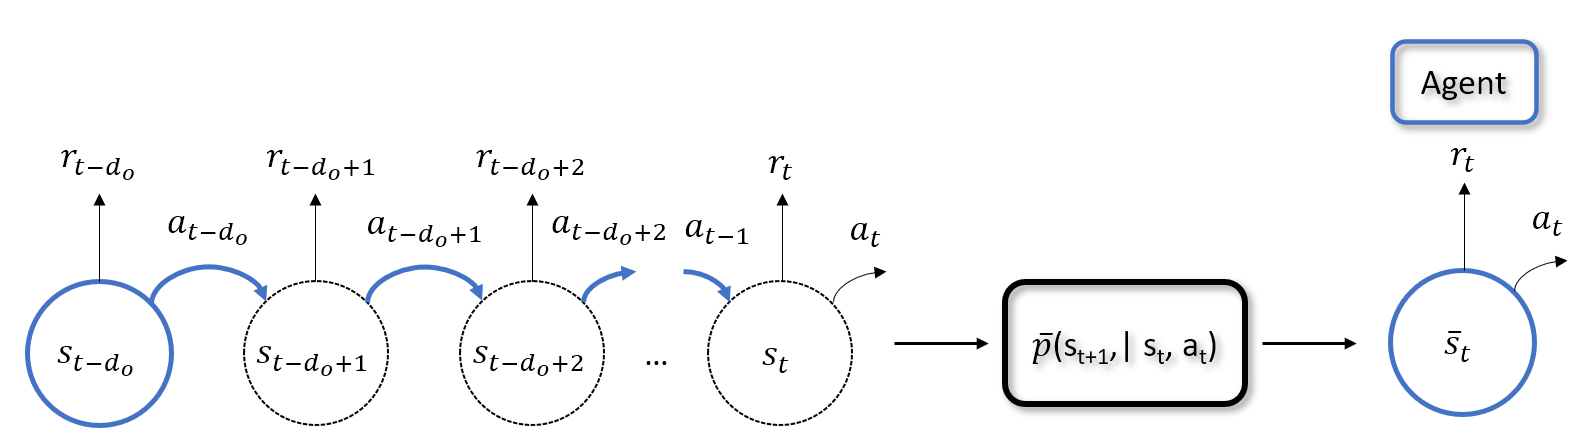
\includegraphics[width=15cm, keepaspectratio]{images/dmdp/modelbased_i_t.png}
                    \caption{Extended State $i_{t}$ is used as source of information to produce a representation $\bar{s}_t$ of the current unobserved state $s_t$, which is considered by the Agent as the current state.}
                    \label{fig:modelbased_i_t}
                \end{figure}
                
                Consider a CDMDP $\langle \mathbf{S}, \mathbf{A}, p, \mathbf{R}, d_o\rangle$. In general, at a certain time-step $t$ the Agent finds itself in an unknown state $s_t$, having available the knowledge contained in the extended state $i_t = \left( s_{t-d_{o}}, a_{t-d_{o}}, ..., a_{t-1}\right)$ and having learnt from some past trajectories an approximation $\bar{p}$ of the state-transition probability function $p$. The information contained in the extended state $i_t$ is then used to infer the current state $\bar{s}_t$ (or a representation of the current state, such as its mean) through the approximation $\bar{p}$. The specific details of the process of computing $\bar{s}_t$ and $\bar{p}$ are the subject of the specific implementation of a Model-Based algorithm, but it is important to notice that $\bar{s}_t$ may not be an element of the State Space $\mathbf{S}$. In fact, it will be referred to only as state "representation", in light of the fact that in more complex situation, such as stochastic environments or stochastic delays, it is impossible to predict an exact state. Once the current state representation $\bar{s}_t$ is available, the Agent is able to select an action $a_t$ based on $\bar{s}_t$ (i.e. $a_t = \pi\left(\bar{s}\right)$) and to execute it. The Agent then finds itself in a new unknown state $s_{t+1}$, it perceives the observation of the old state $s_{t-d_{o}+1}$ and reward $r_t$ and the extended state $i_{t+1} = \left( s_{t-d_{o}+1}, a_{t-d_{o}+1}, ..., a_{t}\right)$ is available to the Agent. Figure \ref{fig:modelbased_i_t} shows the relationship between the extended state $i_t$ and the representation of the current state $\bar{s}_t$.
                \\\\
                As shown in Figure \ref{fig:modelbased_i_t}, Model-Based approach requires the decision making process to be split in two different steps:
                \begin{enumerate}
                    \item\textbf{State Representation:} at first, the knowledge available to the Agent is used to produce representation $\bar{s}_t$ of the current unobserved state $s_t$, possibly with a delay-independent size; 
                    \item\textbf{Action Selection:} then the "usual" action selection and decision-making process is carried out upon the result of the first step, selecting an action $a_t = \pi(\bar{s}_t)$ and executing it.
                \end{enumerate}
                This distinction is very important to describe this approach, because it allows for highlighting the main differences and similarities between Augmented and Memoryless approaches. As in the Augmented approach, Model-Based approach aims to use all the available information at each given time-step $t$, starting from the extended state. However, this information is not used as-is for learning a Policy function or a Value function, instead a current state representation $\bar{s}_t$ is produced. This first step is tackling directly the presence of delays by predicting, possibly meaningful, information about the current state $s_t$. This information is then the input for the second step, which is the usual decision-making with the fundamental difference of being carried out on some representation of $s_t$, possibly not even an actual state of the State Space. As in the Memoryless approach, the decision-making process is void of information about the delay, which is only implicitly expressed in $\bar{s}_t$, at the cost of learning how to produce a meaningful $\bar{s}_t$ from the available knowledge at each time-step $t$.
                \\\\
                The term Model-Based stems from the peculiarities of the State Representation step: in order to produce the current state representation $\bar{s}_t$, the algorithm is forced to learn the dynamics of the environment is some way, thus basing its decisions on a model of the environment. This is in contrast to Model-Free algorithm, where the knowledge of the dynamics of the environment are only implicitly learnt through the set of trajectories that are exploited to find the optimal policy.
                \\\\
                At last, the innovation brought by the Model-Based approach lies in the definition of a new method to execute the State Representation step. Once the State Representation process is defined and working, the Action Selection step can be carried out by any of the state-of-the-art algorithm that already have been presented in the past. In fact, the studies presented in this section are focused on designing a new and more efficient way to produce the state representation, rather than the action selection process. In the same way, the focus of this research work is to define a new structured network (which will be referred to as module in Chapter \ref{chp:ow}), that is able to produce a state representation in different environmental settings. In this research, the Action Selection step is handled by an already defined and presented state-of-the-art algorithm (Section \ref{sota:trpo}).
                
                
            \subsubsection{Model-Based Simulation (MBS)}
                \begin{algorithm}[t]
                    \SetAlgoLined
                    \KwData{CDMDP $M = \langle \mathbf{S}, \mathbf{A}, p, \mathbf{R}, d_o\rangle$; \newline Augmented State $i_t = \left( s_{t-d_{o}}, a_{t-d_{o}}, a_{t-d_{o}+1}, ...,  a_{t-1}\right)$.}
                    \KwResult{Optimal Action for current (unobserved) State: $\pi^{*}(\bar{s}_t)$}
                    Construct an undelayed MDP $\bar{M} = \langle \mathbf{S}, \mathbf{A}, \bar{p}, \mathbf{R}\rangle$.\;
                    Find  $\bar{v}_{*}$ and $\bar{\pi}_{*}$ for $\bar{M}$\;
                    Compute $\bar{s}_t$ by following $\bar{p}$ and the augmented state $i_t$\;
                    Compute the optimal action to be executed in $\bar{s}_t$ according to $\bar{\pi}_{*}$: $\pi^{*}(\bar{s}_t)$.
                    \caption{Model-Based Simulation}
                    \label{algo:mbs}
                \end{algorithm}
                A significant contribution to this approach is given by \pcite{delay:mbs}, which presents Model-Based Simulation (MBS), a planning algorithm that exploits all the relevant concepts along with important theoretical results. \newline
                Given a CDMDP $\langle \mathbf{S}, \mathbf{A}, p, \mathbf{R}, d_o\rangle$, Model-Based Simulation idea is that the information available to the Agent at a given time-step $t$, which is usually summarized in the extended state $i_t = \left( s_{t-d_{o}}, a_{t-d_{o}},..., a_{t-1}\right)$, can be exploited to retrieve an approximation of the current unknown state $s_t$, which will be denoted by $\bar{s}_t$. In order to compute $\bar{s}_t$, MBS constructs a standard MDP $\bar{M} = \langle \mathbf{S}, \mathbf{A}, \bar{p}, \mathbf{R}\rangle$, where $\bar{p}$ is an approximation of the original state-transition function $p$ and it is defined in the following way:
                \[  \bar{p}(s_t, a_t, s_{t+1}) = 1 \] 
                
                \begin{itemize}
                    \item if $s_{t+1}$ is the most likely outcome of executing $a_t$ in $s_t$ in case of a discrete State Space $\mathbf{S}$, or
                    \item if $s_{t+1}$ is the expected outcome in case of a continuous State Space $\mathbf{S}$.
                \end{itemize}
                
                Once $\bar{p}$ is available, the Agent can recursively apply it to the extended state $i_t = \left( s_{t-d_{o}}, a_{t-d_{o}},..., a_{t-1}\right)$ in order to compute the sequence of approximated states $(\bar{s}_{t-d_{o}+1}, \bar{s}_{t-d_{o}+2}, ..., \bar{s}_{t-1}, \bar{s}_{t})$. Finally, the Agent is able to select the next action by assuming that the current state is $\bar{s}_{t}$ and by following the optimal policy obtained by solving $\bar{M}$. The complete algorithm is detailed in Algorithm \ref{algo:mbs}.
                \\\\
                In order to relate to the terminology used in the section \ref{subsubs:mbapproach:general}, the approximation of the current state $\bar{s}_t$ can be considered as a pratical example and implementation of state representation, while $\bar{p}$ is exactly the approximation of the state-transition function $p$. Thus, in the case of Model-Based Simulation, the process that computes the state representation of the current unknown state $s_t$ directly involves an approximation of the state-transition $\bar{p}$ function and it outputs an element of the State Space $\mathbf{S}$.
                \\\\
                Another important contribution given by \pcite{delay:mbs} is the theoretical study about the consequences of the presented approximation. Introducing an approximation also implies introducing a certain amount of error within the discussed algorithm. In practice, the Agent will always act "as if" the current unknown state $s_t$ is exactly its state representation $\bar{s}_{t}$, which is false in general. As a consequence, the optimal action selection cannot be carried out precisely, which in turn results in a loss of performances w.r.t. the undelayed process. However, it is proven that the loss of performances is bounded in case the underlying undelayed dynamics of the environment has the following properties:
                
                \begin{itemize}
                    \item Deterministic and Finite: the undelayed MDP $\langle \mathbf{S}, \mathbf{A}, p, \mathbf{R}\rangle$ is such that $|\mathbf{S}| < \infty$ and $\forall s \in \mathbf{S} \; \exists s' \in \mathbf{S}: \; p(s,a,s') = 1$;
                    \item Deterministic and Continuous: the undelayed MDP $\langle \mathbf{S}, \mathbf{A}, p, \mathbf{R}\rangle$ is such that $\mathbf{S}$ and $\mathbf{A}$ are continuous and $\forall s \in \mathbf{S} \; \exists s' \in \mathbf{S}: \; p(s,a,s') = 1$;
                    \item Mildly Stochastic and Finite: the undelayed MDP $\langle \mathbf{S}, \mathbf{A}, p, \mathbf{R}\rangle$ is such that $|\mathbf{S}| \leq \infty$ and $\exists \delta \leq 0$ such that $\forall s \in \mathbf{S} \; \exists s' \in \mathbf{S}: \; p(s,a,s') \geq 1 - \delta$.
                \end{itemize}
                
                This result is very important because it avoids arbitrarily worse performances w.r.t. the undelayed counterpart, which would greatly impact the applicability of the approach, at the cost of limiting its range of approach.
            
            \subsubsection{A Recurrent Network Algorithm}
                \label{subsub:modelbased_recurrent}            
                \pcite{delay:ssbm} present a Model-Based algorithm in order to cope with the presence of execution delay, using as environment a famous competitive videogame in which the notion of delay is identified as the reaction time an average player is able to express. The proposed algorithm makes use of a Recurrent network based on Gated Recurrent Unit (\pcite{dl:gru}) in order to iteratively predict the sequence of unknown states that are not yet known to the Agent. Given a CDMDP $\langle \mathbf{S}, \mathbf{A}, p, \mathbf{R}, d_a\rangle$, at each time-step $t$ the knowledge contained in the extended state $i_t = \left( s_{t}, a_{t-d_a},..., a_{t-1}\right)$ is available to the Agent. The currently known state $s_t$, denoted from now on as $s_{t, 0}$, is used as input to a GRU along with the core hidden state $h_t$, denoted from now on as $h_{t, 0}$ which is the result of the last iteration of the recurrent network, in order to produce the next core hidden state $h_{t, 1}$ and the core output $o_{t, 0}$. At this point, the triple $(s_{t, 0}, a_{t-d_a}, o_{t, 0})$ is used as input to a learnt state-transition function $\bar{p}$ in order to produce the prediction for the next state, $s_{t, 1}$:
                \[ s_{t, 1} = \bar{p}(s_{t, 0}, a_{t-d_a}, o_{t, 0}) \]
                Once $s_{t, 1}$ is available, it can be used along with $h_{t, 1}$ as input to a GRU in order to produce the next core hidden state $h_{t, 2}$ and the next core output $o_{t, 2}$. The new triple $(s_{t, 1}, a_{t-d_a+1}, o_{t, 1})$ is used to produce $s_{t, 2}$ thorugh $\bar{p}$ and the iteration is repeated. Each step $i$ can be summarized as follows:
                
                \begin{align*}
                    h_{t, i+1}, o_{t, i} &= GRU(s_{t, i}, h_{t, i})\\
                    s_{t, i+1} &= \bar{p}(s_{t, 1}, a_{t-d_a+1}, o_{t, 1})
                \end{align*}
                
                \begin{figure}[b]
                    \centering
                    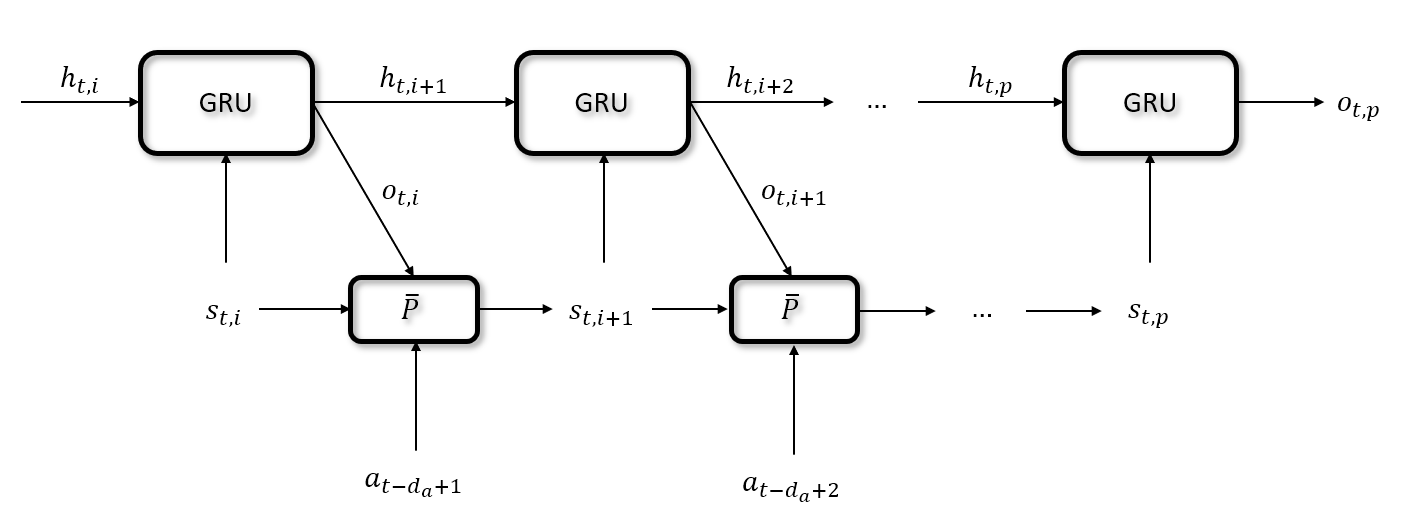
\includegraphics[width=15cm, keepaspectratio]{images/dmdp/modelbased_ssbm.png}
                    \caption{The iterative process of predicting the sequence of states $s_{t, i}$ that will occur in the next $p$ steps along with producing the correspondent core outputs $o_{t, i}$.}
                    \label{fig:modelbased_ssbm}
                \end{figure}
                \noindent
                This iterative process is carried out $p$ times, with $p \leq d_a$ being an hyperparameter of the model. In the last iteration, the core $o_{t, p}$ is produced and used as input to the policy $\pi$ in order to select action $a_t$. As usual, the effect of action $a_{t-d_a+1}$ is observed and the Agent will find itself in the extended state $i_t = \left( s_{t+1}, a_{t-d_a+1},..., a_{t}\right)$. Figure \ref{fig:modelbased_ssbm} provides a visualization of the iterative process that produces the core outputs.
                \\\\
                As it can be observed, the state representation proposed by \pcite{delay:ssbm} is the core output $o_{t,p}$, which is not an element of the State Space $\mathbf{S}$, but rather a vector built by the p-th Gated Recurrent Unit. The idea behind the choice of not using a predicted element of the state space, which is also already available as $s_{t,p}$ in this algorithm, is that it is possible to compress useful information about the current state in a finite vector used as input to the policy $\pi$. In this way, the input space of the policy function is not the State Space $\mathbf{S}$. \newline
                It is important to highlight this concept because it is closely related to the scope of this research, which also tries to compress information about the current state in a finite vector, as it is presented in Chapter \ref{chp:ow}.
                \\\\
                In order for the core output $o_{t,p}$ to represent useful information, the whole network described needs to be trained accordingly. In fact, the predictive model constituted by GRUs and the learnt state-transition probability function $\bar{p}$ is trained against the actual dynamics of the environment: the sequence of predicted states $(s_{t, 1}, s_{t, 2}, $ $..., s_{t, p})$ is compared to the actually experienced sequence of state $(s_{t+1}, s_{t+2}, ..., s_{t+p}$ in a Regression fashion. In this way, the core hidden state $h$ and core output $o$ are driven towards compressing useful information about the current unknown state $s_{t+d_a}$ in which the Agent will execute the chosen action $a_t$. In practice, the network learns to predict the most probable state starting from $h$ and $o$. In this regards, experiments have highlighted how the best choice of the hyperparameter $p$ is exactly the execution delay $d_a$. This is also intuitively reasonable: in the case in which $p = d_a$, at each time-step, the Agent is trained on the entire sequence of states that separates it from the state in which it will execute action $a_t$, thus resulting in a more accurate prediction $s_{t, p}$, which in turn is translated in a more meaningful core output $o_{t, p}$. The other two possible cases are: $p < d_a$, the Agent never learns to predict the current state $s_t$ and its estimates refers to an earlier, different, state $s_{t,p}$; $p > d_a$, the Agent learns to predict more states than necessary, making the overall network more complex and the $s_{t, d_a}$ prediction less accurate. These conclusions are also confirmed by the results of this research shown in Section \ref{sub:res_test_delays}.
                
            \subsubsection{Model-Based Approach for Stochastic Delays} 
                \begin{figure}[t]
                    \centering
                    
                    \begin{subfigure}[b]{.45\textwidth}
                        \centering
                        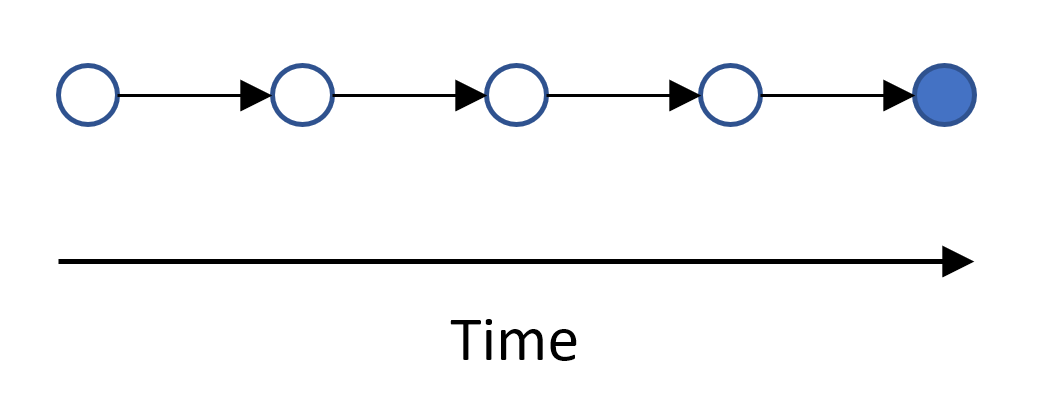
\includegraphics[width=\textwidth]{images/dmdp/modelbased_stochastic_1.png}
                        \caption{Deterministic delay in a deterministic environment.}
                        \label{fig:modelbased_stochastic_1}
                    \end{subfigure}
                    \hfill
                    \begin{subfigure}[b]{.45\textwidth}
                        \centering
                        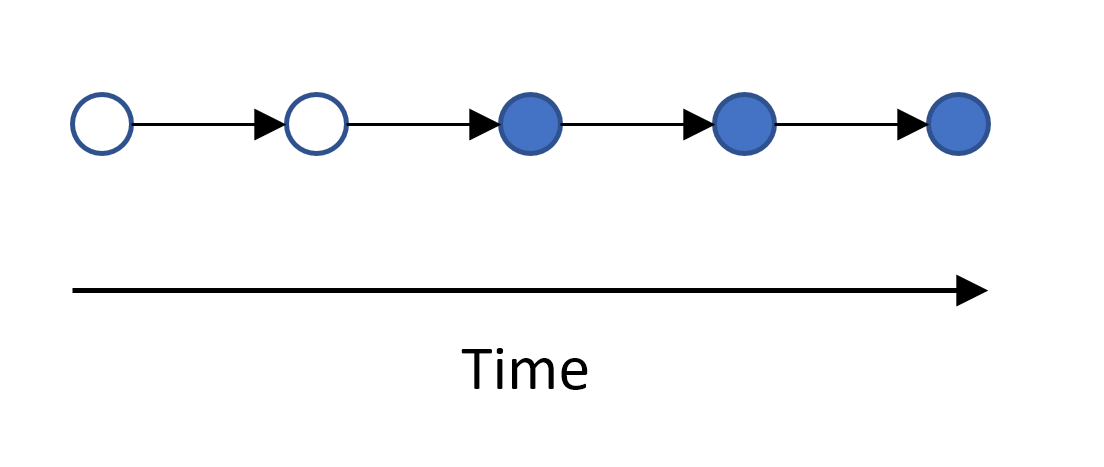
\includegraphics[width=\textwidth]{images/dmdp/modelbased_stochastic_2.png}
                        \caption{Stochastic delay in a deterministic environment.}
                        \label{fig:modelbased_stochastic_2}
                    \end{subfigure}
                    
                    \begin{subfigure}[b]{.45\textwidth}
                        \centering
                        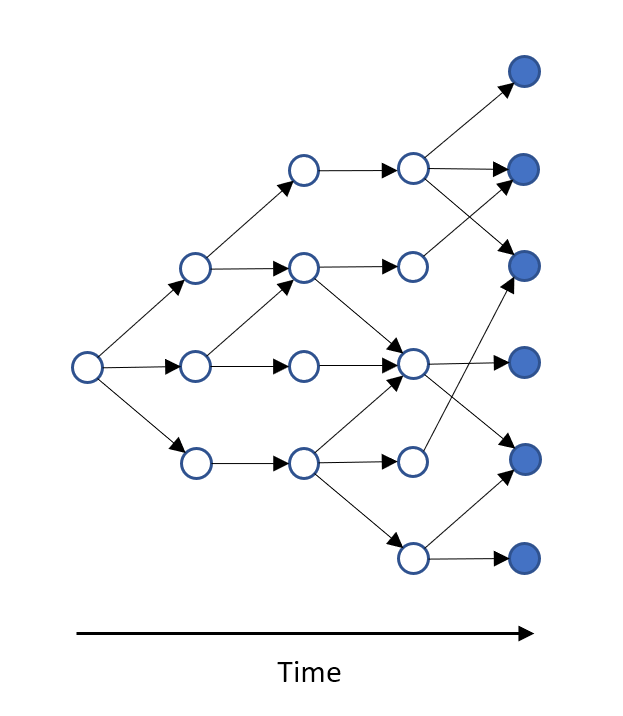
\includegraphics[width=\textwidth]{images/dmdp/modelbased_stochastic_3.png}
                        \caption{Deterministic delay in a stochastic environment.}
                        \label{fig:modelbased_stochastic_3}
                    \end{subfigure}
                    \hfill
                    \begin{subfigure}[b]{.45\textwidth}
                        \centering
                        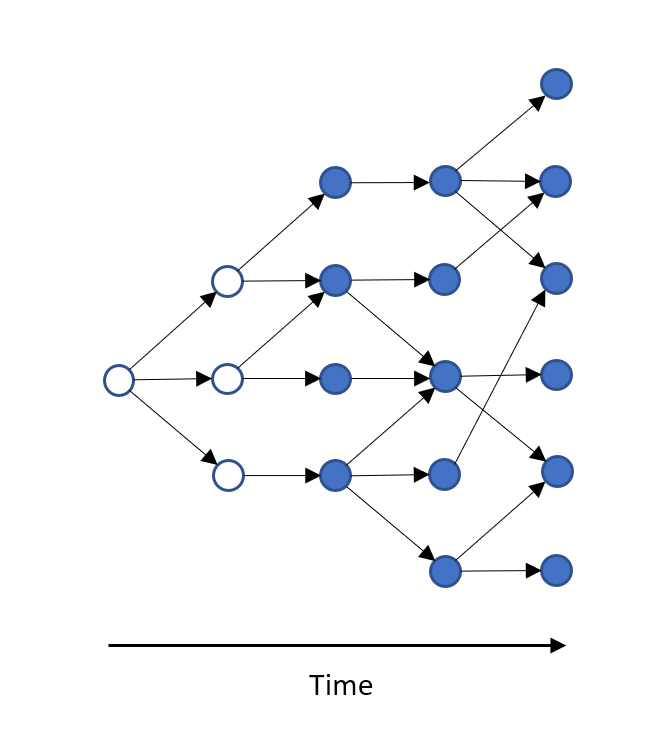
\includegraphics[width=\textwidth]{images/dmdp/modelbased_stochastic_4.png}
                        \caption{Stochastic delay in a stochastic environment.}
                        \label{fig:modelbased_stochastic_4}
                    \end{subfigure}
                    
                    \caption{An example of how stochasticity impact the current unknown state distribution. In each figure, each circle represents a state and each arrows an action. The Agent last known state is the left-most state. The other white states are states that could have been reached by the Agent, while the blue states are states in which the Agent could be now. Both white states and blue states are unknown because the presence of delays.}
                    \label{fig:modelbased_stochastic}
                \end{figure}
            
                Throughout the previous paragraphs delay is assumed constant so to focus on other relevant aspects of the approach. Nevertheless, important observations can be made for the case of stochastic delays. Given the definition of Model-Based approach presented in Section \ref{subsubs:mbapproach:general}, the impact of stochasticity in the delay process $d_o(t)$ affects only the State Representation step, since the extended state $i_t$ will contain a variable number of actions depending on the sampled delay at time-step $t$. The fact that $i_t$ has a variable number of actions actually has a huge impact from different point of views, especially in the design of the algorithm. \newline
                The structured component that implements the State Representation step needs to be able to cope with a variable length input in some way. Accepting inputs of different lengths at each step is not a trivial task: for example, standard neural networks are not able to manage such inputs, while recurrent networks such as GRU or Long-Short Term Memory (LSTM, \pcite{dl:lstm}) are capable of handling them, but with a computational cost that increase in the length of the input. From the learning difficulty point of view, the context of stochastic delays is much more complex: the model needs to be able to output relevant state representations not only for fixed amount of steps in the future, but for different amounts, at once. \newline
                The State Representation $\bar{s}_t$ is directly used as input for the Action Selection step. In the case of stochastic delays, it is not trivial to design the size of $\bar{s}_t$: if the structured network that computes it  mantains its variable length, then the variable length issue is propagated to the Action Selection step, thus to the policy function. On the other hand, having a fixed length $\bar{s}_t$ means that information about the current state distribution is compressed on a fixed length vector, which still needs to be able to contain a relevant amount of information so that the Action Selection step can achieve good performances overall. \newline
                At last, Figure \ref{fig:modelbased_stochastic} shows the differences between the deterministic delay and the stochastic delay cases, along with deterministic and stochastic environment. Intuitively, the case of deterministic delays in a deterministic environment is the easiest to solve and knowing the dynamics of the environment perfectly leads to solving the State Representation step in a closed form: applying each action recursively to the last known state would always generate the exact sequence of states that will be perceived by the agent in the future. In practice, there is no other state in which the Agent could be. The presence of stochasticity can greatly complicate this setting, since the currently unknown state could greatly vary both in the Stace Space $\mathbf{S}$ and in the time-step $t$, leading to a more elaborated probability distribution and, in turn, to a much more complex state-transition probability function which needs to be learnt by the Agent. 
                
            \subsubsection{Advantages and Disadvantages}
                Advantages and disadvantages of the Model-Based approach stem from the comparison against the other two approaches presented so far. In fact, as said in the introduction, the Model-Based approach represents a middle ground between the Augmented and Memoryless approach, focusing on escaping the inherent complexity of the first while incorporating more knowledge of the delay w.r.t. the second. 
                \\\\
                As stated in Theorem \ref{th:dmdpobscomplexity}, the Augmented approach heavily suffers from the computational complexity point of view: incorporating the knowledge of the delay directly within the state of the new augmented MDP to be learnt has the side effect of making it solvable in exponential time w.r.t. the amount of delay, as proven by \pcite{delay:mbs}. Instead, the Model-Based approach is able to incorporate knowledge about delays escaping the exponential time complexity: the Agent learns upon a representation of the current state $\bar{s}_t$, which can be designed to be of fixed size regardless of the amount of delay present. Thus, this class of algorithms is able to solve the original DMDP in polynomial time, as demonstrated by \pcite{delay:mbs}. As usual, this advantage does not come for free: the Model-Based approach needs to learn the dynamics of the underlying DMDP and the higher the amount of delay, the more difficult is the task, as shown in Figure \ref{fig:modelbased_stochastic}.
                \\\\
                At the same time, Model-Based approach cannot be as fast as Memoryless approach in general, exactly because of its need of learning the dynamics of the underlying MDP. As the result of this research will show, also Model-Based algorithms suffer from optimizing towards suboptimal solutions, but the underlying hypothesis is that they offer a better trade-off between computational complexity and integrating knowledge about delays, thus leading to better solutions.
                \\\\
                As explained in previous sections, designing a Model-Based algorithm requires important decision-making towards the State Representation step, specifically about which kind of networks are suitable for the scope of the algorithm and thus which are the delay and environment properties that can be handled by the algorithm. In other words, the State Representation step answers to the question of how can the information available to the Agent be used efficiently in order to produce a meaningful information vector that is then used as input for the Action Selection step. This approach allows for improving or changing the State Representation step without affecting the Action Selection step, which can be carried out by past, current or even future state-of-the-art algorithms. Thus, another important advantage of the Model-Based approach is the wide applicability with existent or future RL algorithms.
                
                % \begin{figure}
                %     \centering
                    
                %     \vspace{1.0cm}
                %     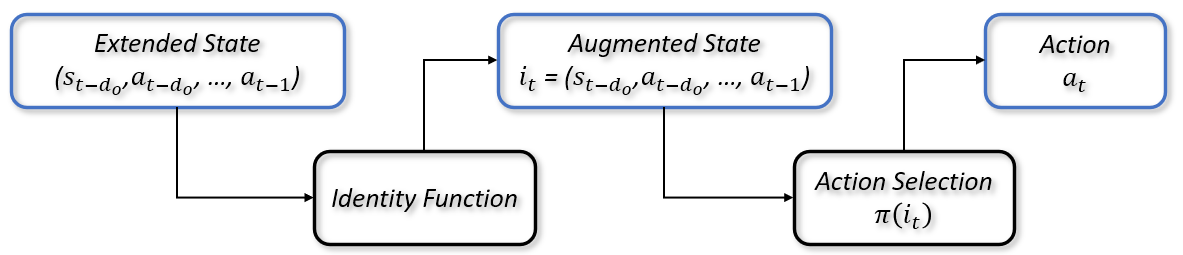
\includegraphics[width=15cm, keepaspectratio]{images/dmdp/modelbased_appr_augmented_2.png}
                %     \caption{Augmented Approach presented as a particular case of Model-Based Approach. Knowledge available or inferred by the Agent is highlighted in light blue and computational steps are highlighted in black. State Representation's black box is an identity function, while Action Selection is the usual decision-making choice.}
                %     \label{fig:modelbased_appr_augmented}
                    
                %     \vspace{2.5cm}
                    
                %     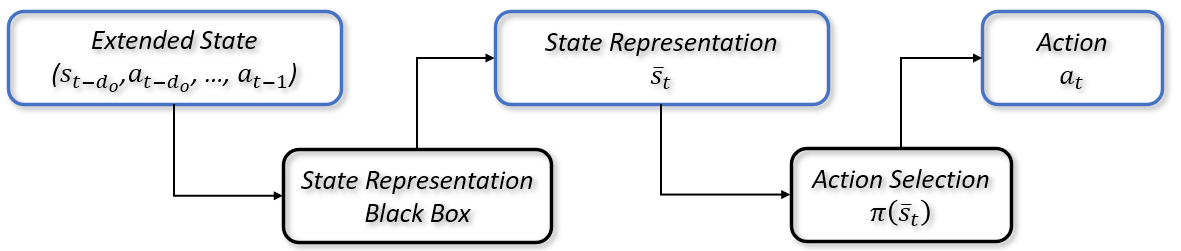
\includegraphics[width=15cm, keepaspectratio]{images/dmdp/modelbased_appr_modelbased_2.png}
                %     \caption{Model-Based Approach presented as sequence of steps, knowledge available or inferred by the Agent is highlighted in light blue, while computational steps are highlighted in black. State Representation is described as a black box, while Action Selection is the usual decision-making choice.}
                %     \label{fig:modelbased_appr_modelbased}
                    
                %     \vspace{2.5cm}
                    
                %     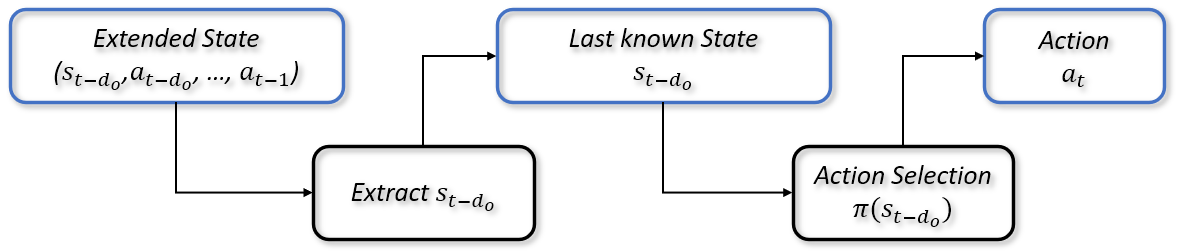
\includegraphics[width=15cm, keepaspectratio]{images/dmdp/modelbased_appr_memoryless_2.png}
                %     \caption{Memoryless Approach presented as a particular case of Model-Based Approach. Knowledge available or inferred by the Agent is highlighted in light blue and computational steps are highlighted in black. State Representation's black box only extracts the last known observation from the extended state, while Action Selection is the usual decision-making choice.}
                %     \label{fig:modelbased_appr_memoryless}
                %     \vspace{1.0cm}
                % \end{figure}
        
    \newpage
    \section{Partially Observable MDP}
        \label{sota:pomdp}
        % Section Schema
        % Introduction on POMDP citing Chapter 2 Section on Belief
        %   - Subsection: Link between DMDP and POMDP (extendedstate as observation)
        %   - Subsection: PSD
        %   - Subsection: RPSP
        %   - Subsection: Link between RPSP and Model-Based Approach + Advantages
        
        This section is dedicated to present the similarities between the Delay MDP framework and the Partially Observable MDP framework. Establishing a link between the two frameworks allows for also establishing a connection between the correspondent literatures. Since DMDP research is far less explored than POMDP research, this process is especially beneficial for first. In fact, two specific studies in POMDP research are presented as they have been important in the process of developing this research original work: Section \ref{subs:psd} is focused on Predictive-State Decoder (PSR) architecture, which introduces the idea of evaluating the network using a second performance measure to drive the internal state of the network towards a meaningful quantity; while Section \ref{subs:rpsp} presents Recurrent Predictive-State Policy networks, a direct application of the PSR paradigm.
        
        \subsection{Connection between DMDP and POMDP}
            In Section \ref{subs:pomdp}, the concepts of Observation function and Belief have been presented and they can be expanded further now, after having presented the different DMDP approaches in Section \ref{sota:delay_approaches}. The core issue of POMDP framework is that, at each time-step $t$, the Agent perceives an observation $o_t$ of the current state $s_t$ and the relationship between observations and states is not one-to-one: observing $o_t$ may be resulting from several states $s_t$. Thus the Agent needs to plan its actions not only according to the dynamics of the environment, but also understanding them through incomplete observations. The concept of observation is generic in the literature, since it may represent any information that the Agent is able to perceive from the current state of the environment.
            \\\\
            While the terminology is different, the class of DMDP Agents under Memoryless and Model-Based approaches are actually working under the same assumption of POMDP Agents: at each time-step $t$, the Agent perceives partial information of the extended state $i_t = (s_{t-d_o}, a_{t-d_o}, ..., a_{t-1})$, thus matching the definition of observation. The differences lie in how the Agent makes use of the extended state $i_t$, i.e. which information is extracted and reasoned upon, thus in which approach is taken by the agent.
            
            \subsubsection{Memoryless Approach as POMDP}
                Memoryless approach does not fully utilize the extended state $i_t$, as explained in Section \ref{subs:memorylessapproach}. Regardless of the fact that other mechanism in the algorithm may be able to use information about the presence of delay, the Agent's observation is the last known state: $o_t = s_{t-d_o}$. As in the previous section, it is possible to specifically define the Observation function $O$ for the Memoryless approach:
                
                \[ O(s_t|o_t) = O(s_t|s_{t-d_o}) = \sum_{i = t - d_o}^{t-1} \sum_{a \in \mathbf{A}} p(s_{i+1}|s_{i}, a)\]
                
                where $p$ is the state-transition probability function of the environment. Thus, a Belief of the current unknown state $s_t$ can be defined. \newline
                Furthermore, it is possible to observe that Memoryless approach is actually a solution directly borrowed from the POMDP literature, where Memoryless algorithms are algorithms that makes only use of the last known observation $o_t$ in order to plan the next action. In the same way, Memoryless policy makes only use of the last known state $s_{t-d_o}$ in order to plan the next action.
            
            \subsubsection{Model-Based Approach as POMDP}
                As explained in Section \ref{subs:modelbasedapproach}, the Agent's decision-making process is split into two different steps: the result of the State Representation step can be thought as the observation $o_t = f (i_t)$, where $f$ is a function that implements the State Representation step itself, that the Agent actually perceive and which is then used by the Action Selection step to chose the next action $a_t$. \newline
                Thus, it is of interest for Model-Based approach research to look into the POMDP research for new solutions and concepts that may help to develop new and more efficient algorithms and for this reason the next sections are focused on presenting results from the POMDP literature that have been helpful towards the development of this research's original work.
                
        \subsection{Predictive-State Decoders}
            \label{subs:psd}
            \pcite{pomdp:psd} expands on the existing solution of using Recurrent Neural Networks (RNN) for dealing with POMDP framework, presenting a new architecture called Predictive-State Decoder, which is specifically designed to cope with the main issues of the Recurrent models. 
            
            \subsubsection{Recurrent Models}
                Recurrent Neural Networks have been proposed as a solution to Partially Observable MDP due to their ability of maintaining and updating an internal state, denoted $h_t$, at each time-step $t$. In general, the main objective of Recurrent models is to find a model $f$ that receives as input the last observation $o_t$ and it is able to recursively update its internal state $h_t$ while predicting a target variable $y_t$. The sequence of target variables is then collected and used to compute the Loss Function $L$, through which the recurrent network is optimized:
                
                \[ \min_{f} L = \min_{f} \sum_{t} l(f(h_t, o_t)) \]
                
                \noindent
                This process is illustrated in Figure \ref{fig:pomdp_rnn}. In POMDP framework, Recurrent models have the objective of selecting the next action $y_t = a_t$ while updating the current internal states $h_t$ and the underlying assumption is that by optimizing the whole network towards the optimal performance w.r.t. the collected rewards, the internal state updates will eventually lead $h_t$ to a meaningful representation of the current unknown state. In practice, as \pcite{pomdp:psd} observe, the absence of a loss function directly specified over $h_t$ makes this task very difficult to achieve and a Recurrent model that does not encode meaningful information within its internal state is bound to perform poorly.
                
                \begin{figure}[t]
                    \centering
                    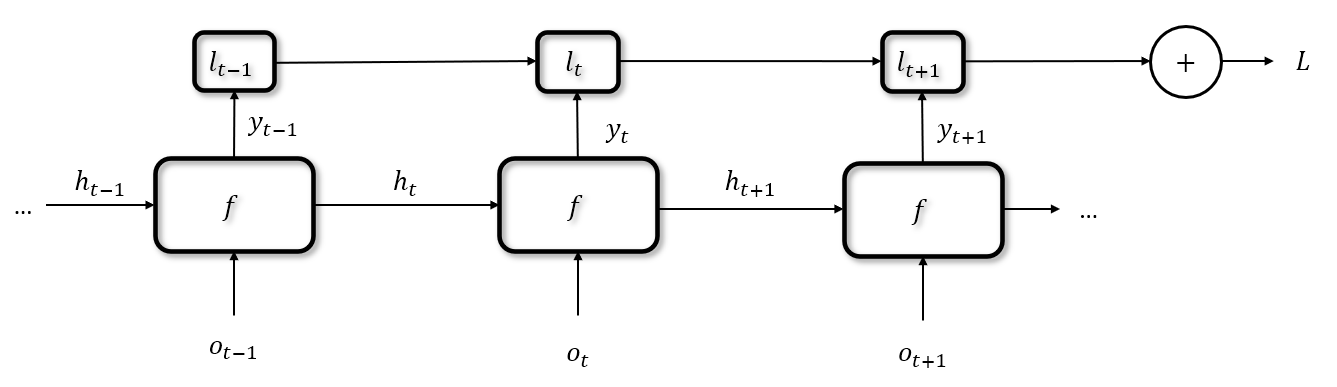
\includegraphics[width=15cm, keepaspectratio]{images/pomdp/pomdp_rnn.png}
                    \caption{Recurrent model. At each time-step $t$, the model $f$ receives as input the previous internal state $h_{t-1}$ and the latest observation $o_{t-1}$ in order compute the next internal state $h_{t}$ and the prediction $y_{t}$. The prediction $y_t$ is then used to compute the current loss $l_t$. All losses $l_t$ are summed together to retrieve Loss function $L$.}
                    \label{fig:pomdp_rnn}
                \end{figure}
                
            \subsubsection{Predictive-State Decoders}
                The solution proposed by \pcite{pomdp:psd} is to add a new portion to the recurrent architecture that is dedicated to evaluate the internal states during the training process. Its purpose is to assess how much the internal state is close to a meaningful target variable: the sequence of future observations $(o_{t+1}, o_{t+2}, ...)$. This evaluation is then added to the Loss function through which the entire architecture is optimized. This allows for finding an internal state $h_t$ only by means of quantities observed by the Agent during its interaction with the environments. The class of methods that allows for this behaviours is called Predictive-State Representations (PSR). \newline
                In practice, at each time-step $t$, the L2-Norm between $h_t$ and the sequence of future observation $(o_{t+1}, o_{t+2}, ..., o_{t+d})$ is computed. In order to be able to compute the L2-Norm starting from arbitrary sizes of $h_t$, an encoder $F$ is added. The sequence of L2-Norm computed at each time-step $t$ is then collected to form a new loss Function, the Predictive-State loss function:
                
                \begin{definition}[Predictive-State Loss function $R$]
                    \[ R = \sum_{t=0}^{T} \| F(h_t) - \phi([o_{t+1}, o_{t+2}, ..., o_{t+d}])\|^{2}\]
                    
                    where $\phi$ denotes some feature functions chosen for the future observations.
                \end{definition}
                
                \noindent
                The Predictive-State loss function $R$ is then weigthed by a factor $\lambda$ and added to the previously defined loss function:
                
                \[ \mathbb{L} = L + \lambda R\]
                
                where $\lambda$ is used to tune the importance of $R$ within the entire loss function. This architecture is called Predictive-State Decoder (PSD) and it is shown in Figure \ref{fig:pomdp_psd}. 
                
                \begin{figure}[!t]
                    \centering
                    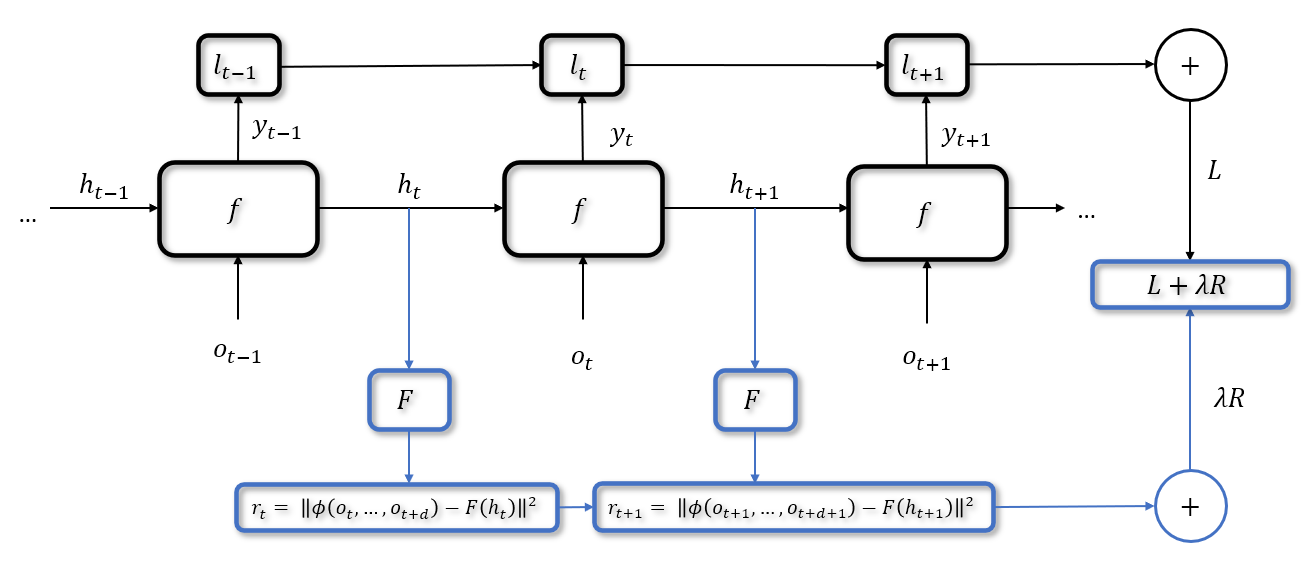
\includegraphics[width=15cm, keepaspectratio]{images/pomdp/pomdp_psd.png}
                    \caption{Predictive-State Decoder, the differences with the Recurrent model are highlighted in light blue. In addition to the Recurrent model, at each time-step $t$, the internal state $h_t$ is first encoded through $F$ and then used to compute the current Predictive-State loss $r_t$. All Predictive-State losses $r_t$ are summed together to retrieve the Predictive-State loss $R$, which is then weighted by $\lambda$ and added to $L$.}
                    \label{fig:pomdp_psd}
                \end{figure}
                
            \subsubsection{Multi-Task Learning}
                Predictive-State Encoder architecture can be interpreted as an example of Multi-Task Learning (MTL, \pcite{ml:mtl}). Multi-Task Learning is a particular instance of Machine Learning methods that are able to learn upon different tasks at the same time, with the purpose of improving the overall performances of algorithm by letting the different tasks interact together. In the Predictive-State Decoder example, the Agent is both learning how to optimize the action selection process towards higher rewards and a meaningful internal state $h_t$. This two tasks are not completely independent, in fact the underlying hypothesis is that driving $h_t$ towards the representation of meaningful information will lead to a better action selection. This type of Multi-Task Learning is important for the scope of this research, since its concepts provided guidance for part of the design or the original work.
                
        \subsection{Recurrent Predictive State Policy Networks}
        \label{subs:rpsp}
            A step forward in the research on Predictive-State Representations and Multi-Task Learning for POMDP is taken by \pcite{pomdp:rpsp}, who present a complete and structured network called Recurrent Predictive State Policy (RPSP). \newline
            RPSP network is divided into two main components with their distinct set of parameters that interact together: the first component is a Recurrent Predictive-State Representation network that is able to produce predictions of the next observations and to update its internal states; the second component is a stochastic parameterized policy that is able to map the internal states to a distribution over the actions. Both these components are described in the following sections.
            
            \subsubsection{Predictive-State Representation}
                The Predictive-State Representation component is the recurrent component of the architecture. Its purpose is to update the internal state $q_t$ and to output a prediction of the next observation $\bar{o}_t$, which is then used to compute the Predictive loss upon which the component is optimized. In order to achieve both objectives, the set of parameters of the PSR component $\theta_{PSR}$ is divided in two sets, $\theta_{ext}$ for updating the internal state and $\theta_{pred}$ for computing the predicted observation. \newline
                The purpose of updating the internal state $q_t$ is to encode a precise quantity: the conditional distribution of future observations conditioned on the correspondent future actions. For this reason, $q_t$ is also denoted as Predictive State. Its update is computed as follows:
                
                \[  q_{t+1} = f_{cond}(\theta_{ext} q_t, a_t, o_t) \]
                
                where $a_t$ is the last action chosen, $o_t$ is the last observation perceived and $f_{cond}$ is a conditioning function chosen beforehand. In their work, \pcite{pomdp:rpsp} also provides a sound procedure to initialize $\theta_{ext}$ and update it during the learning process.
                \\\\
                In order to compute the prediction of the future observation $\bar{o}_t$, the other set of parameters $\theta_{pred}$ is used along with the action chosen by the policy $a_t$ and the current predictive state $q_t$:
                \[ \bar{o}_t = \theta_{pred} (q_t \times a_t)\]
                The purpose of computing $\bar{o}_t$ is that it is possible to define a loss function $l_2$ over the estimation error w.r.t. the actual $o_t$. Including this loss function as a component of the complete loss function $L$ allows for driving the predictive state $q_t$ towards the interpretation of the conditional future observations. The loss function $l_2$ is defined as follows:
                \[ l_2 = \sum_{t=0}^{T} \mathbf{E}_{\rho(\tau|\theta_\pi)} \left[ \| \bar{o}_t - o_t \|^2 \right]\]
                where the expectation is taken over the probability distribution of the trajectories under the current policy.
            
            \subsubsection{Recurrent Predictive State Policy (RPSP)}
                The structure of the parameterized policy $\pi$ is strictly dependent on the Predictive-State Representation component. At each timestep $t$, the policy input is the internal state $q_t$ which is recursively updated by PSR. Under the assumption of a Gaussian distribution $\mathcal{N}(\mu_{t}, \sigma_{t}^{2})$ for the actions, the structure of the network is composed of a feedforward neural network $\varphi$, with a set of parameters denoted as $\theta_{mean}$, which computes the mean of the distribution, and a learnable parameter $\theta_{var}$, upon which the variance of the distribution is computed. These two sets of parameters are combined to form the set of policy parameters $\theta_\pi$. Once $\mu_{t}$ and $\sigma_{t}^{2}$ are available, the policy can sample the gaussian distribution $\mathcal{N}$ in order to provide the next action $a_t$. To summarize the process:
                
                \begin{align*}
                    \mu_{t} &= \varphi(\theta_{mean}, q_t)\\ \sigma_{t}^{2} &= \text{diag}(\text{exp}(\theta_{var}))^{2}\\
                    a_t &= \text{Sample}(\mathcal{N}(\mu_{t}, \sigma_{t}^{2}))
                \end{align*}
                
                where $q_t$ is the internal state of the PSR component, $diag$ and $exp$ represent respectively the usual diagonal and exponential operators. \newline
                The loss function defined over the policy parameters $\theta_\pi$ is denoted as $l_1$ is the usual expected returns for an Agent that follows a policy with parameters $\theta_\pi$:
                \[ l_1 = -J(\theta_\pi)\]
            
            \subsubsection{RPSP Network}
                At last, it is now possible to present the schema of the entire architecture, illustrated in Figure \ref{fig:pomdp_rpsp}. In order to learn the RPSP $\pi_\theta$, the proposed algorithm seeks to minimize the following objective function:
                \[ L(\theta) = \alpha_{1} l_1 + \alpha_{2} l_2 = - \alpha_1 J(\theta_\pi) + \alpha_2 \sum_{t=0}^{T} \mathbf{E}_{\rho(\tau|\theta_\pi)} \left[ \| \bar{o}_t - o_t \|^2 \right]\]
                where $\alpha_1, \alpha_2 \in \mathbb{R}$ are hyperparameters used to tune the relative importance of the $l_1$ and $l_2$. Given that the loss function $L$ is divided into two distinct component by design, \pcite{pomdp:rpsp} proposes two different optimization algorithms for each of them, in order to retrieve the estimate of their gradient w.r.t. the parameter vector $\theta$ and compute the overall update through a gradient descent update. In practice:
                \begin{itemize}
                    \item Loss function $l_1$: the gradient of $l_1$ w.r.t. $\theta$ can be retrieved by means of Policy Gradient methods or Actor-Critic methods (Section \ref{subs:policygrad_actorcritic}), such as REINFORCE (\pcite{REINFORCE}) or Trust Region Policy Optimization (Section \ref{sota:trpo}).
                    \item Loss function $l_2$: the gradient of $l_2$ w.r.t. $\theta$ can be retrieved by means of Backpropagation Through Time.
                \end{itemize}
                \noindent
                The contribution of \pcite{pomdp:rpsp} is important to the scope of this research because it defines a complete and implementable algorithm that solves POMDP problems through Multi-Task Learning and exploiting recent algorithms of interest such as Trust Region Policy Optimization. As it will be explained in Chapter \ref{chp:ow}, these characteristics have been an inspiration for the development of the original work.
                
                \begin{figure}[t]
                    \centering
                    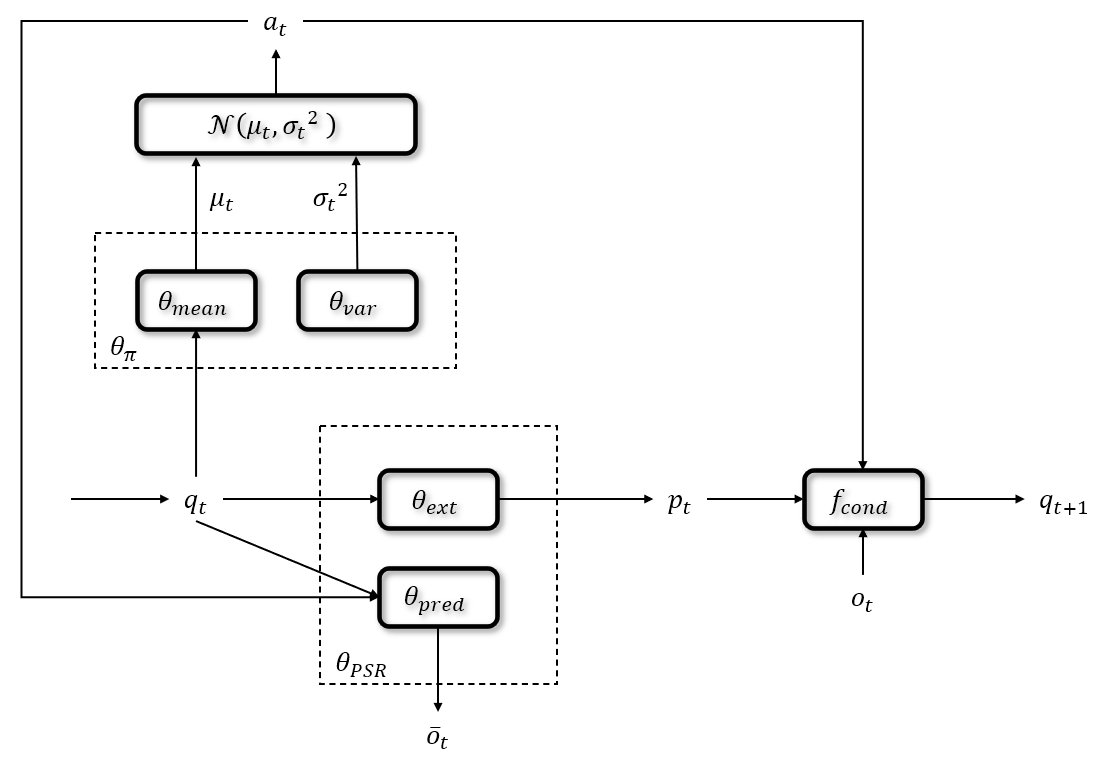
\includegraphics[width=15cm, keepaspectratio]{images/pomdp/pomdp_rpsp.png}
                    \caption{Recurrent Predictive State Policy network schema.}
                    \label{fig:pomdp_rpsp}
                \end{figure}
                
        \newpage        
        \subsection{DMDP Advantages over POMDP}
            In this section, the similarities between DMDP and POMDP frameworks have been highlighted, along with two architectures and two algorithms that aims to overcome the primary issues of exploiting Recurrent networks to solve POMDP problems. The fact that DMDPs can be seen as a particular case of POMDPs is very helpful towards the DMDP research field: POMDP research becomes a source of concepts, ideas and algorithms that could improve the DMDP state-of-the-art algorithms, while DMDP research remains scarce in general. At the same time, it highlights how DMDP problems may be as complex as POMDP problems in general. \newline
            However, DMDP framework has one significant advantage. Due to the fact that in the POMDP framework states of the environment are not usually available, POMDP algorithms based on Predictive-State Representation models are forced to predict observations $o$ rather than states, while DMDP algorithms have access to the exact state $s$ after a certain number of steps, decided by the amount of delay present. At training time, Model-Based DMDP algorithms are able to optimize their state representations $\bar{s}$ by using the exact knowledge of the actually visited states $s$, rather than an inexact observation: it suffices to draw some trajectories using the currently learnt policy, collect the actually visited states and realign them with their correspondent prediction states. This procedure has already been tested by other researches such as \pcite{delay:ssbm}, discussed in Section \ref{subsub:modelbased_recurrent}, and the current research is based on the hypothesis that it is worth investigating in this direction in order to formulate new algorithms to solve the DMDP problems.
            